%\documentclass[aastex,a4paper,12pt]{book}
\documentclass[a4paper,11pt]{report}
\usepackage[T1]{fontenc}
\usepackage[utf8]{inputenc}
\usepackage{lmodern}
\usepackage[spanish]{babel}
\usepackage[dvips]{graphics,color,epsfig}
%\usepackage[latin1]{inputenc}

\usepackage{pst-all}
\usepackage{pstricks}

\usepackage{amssymb} % Math
\usepackage{graphicx}
\usepackage{float}
\usepackage{amsmath}
%

% Defino clases de secciones en ESPAÑOL
\def\chaptername{Cap\'\i tulo}
\def\abstractname{Resumen}
\def\contentsname{Contenidos}
\def\bibname{Bibliograf\'\i a}
\def\appendixname{Ap\'endice}
\def\tablename{\textbf{Tabla}}
\def\figurename{\textbf{Figura}}
\usepackage[dvips]{graphics,color,epsfig}
\usepackage{pst-all}
\usepackage{pstricks}
%\usepackage[spanish]{babel}
\usepackage[spanish,es-nodecimaldot]{babel}
\topmargin=-2cm  

\addto\captionsspanish{\def\tablename{Tabla}}


%Paquetes a utilizar
\input{epsf.sty}

\usepackage{amssymb}
%\usepackage[spanish]{babel}
\usepackage[utf8]{inputenc}

\usepackage{amssymb} % Math
\usepackage{graphicx}
\usepackage{float}
%\usepackage{wrapfig}
%\usepackage{deluxetable}

\pagenumbering{arabic}
\usepackage[dvips]{graphics,color}
\usepackage{amssymb} % Math
\usepackage{amsmath} % Math
%\usepackage{dsfont} % Math
\usepackage{float}
\usepackage{graphicx}
\usepackage{wrapfig}
\usepackage{pst-all}
\usepackage{multirow} % Multi filas
\usepackage{multicol}

\usepackage{anysize}
\marginsize{3cm}{3cm}{3cm}{3cm}
\linespread{1.3}

\usepackage{natbib}

%Separacion silabica:
%\usepackage[T1]{babel} % silabas y hyphenation
%\hyphenation{e-vi-den-cia}
%\hyphenation{an-te-rio-res}

% Control de Márgenes

% NAHUEL's
\setlength{\oddsidemargin}{0.5cm}
\setlength{\evensidemargin}{1.5cm}
\setlength{\topmargin}{2cm}
%\setlength{\headheight}{1cm}
%\setlength{\headsep}{1cm}
%\setlength{\topskip}{1.5cm}
\setlength{\textheight}{20cm}
\setlength{\textwidth}{16cm}
%\setlength{\parindent}{1em} % sangria

% ALBERT's
\usepackage{anysize}
\marginsize{2.cm}{2.cm}{0.5cm}{0.75cm} %{left}{right}{top}{bottom}
\marginsize{3.cm}{2.cm}{2cm}{3cm} %{left}{right}{top}{bottom}

\newcommand{\HRule}{\rule{\linewidth}{0.5mm}}

%Font Arial
%\renewcommand{\rmdefault}{phv} % Arial
%\renewcommand{\sfdefault}{phv} % Arial

% Math:
\def\deg{$^\circ$}
\def\rsun{R$_{\odot}$}
\def\bB{\mathbf{B}}
\def\bE{\mathbf{E}}
\def\dpar#1#2{\frac{\partial#1}{\partial#2}}
%color:
\def\red#1{{\textcolor{red}{#1}}}
\def\azul#1{{\textcolor{blue}{#1}}}

\def\fig#1{Figura \ref{#1}}
\def\figa#1#2{Figuras \ref{#1} a \ref{#2}}
\def\figsy#1#2{Figuras \ref{#1} y \ref{#2}}
\def\tabla#1{Tabla \ref{#1}}
\def\eq#1{Ecuaci\'on (\ref{#1})}
\def\eqa#1#2{Ecuaciones (\ref{#1})-(\ref{#2})}
\def\eqn#1{Ecuaci\'on (\ref{#1})}
\def\eqsy#1#2{Ecuaciones (\ref{#1}) y (\ref{#2})}
\def\seccion#1{Sección \ref{#1}}
\def\cap#1{Capítulo \ref{#1}}

\def\exp{{\rm exp}}
\def\ln{{\rm ln}}
\def\sin{{\rm sen}}
\def\cos{{\rm cos}}
\def\sec{{\rm sec}}
\def\erg{{\rm erg}}
\def\cm{{\rm cm}}
\def\km{{\rm km}}
\def\sr{{\rm sr}}
\def\Hz{{\rm Hz}}
\def\GHz{{\rm GHz}}
\def\kev{{\rm kev}}
\def\sfu{{\rm SFU}}
\def\K{{\rm K}}
\def\MK{{\rm MK}}
\def\AU{{\rm UA}}
\def\UA{{\rm UA}}
\def\Log10{{\rm log_{10}}}
\def\G{{\rm G}}
\def\gsun{g_{\odot}}
\def\Rsun{R_{\odot}}
\def\Msun{ M_{\odot}}
\def\Ne{N_\mathrm{e}}
\def\NH{N_\mathrm{H}}
\def\NHe{N_\mathrm{He}}
\def\me{m_\mathrm{e}}
\def\mH{m_\mathrm{H}}
\def\mHe{m_\mathrm{He}}
\def\Tm{T_m}
\def\Tfit{T_{\rm fit}}
\def\Tefit{T_{e,{\rm fit}}}
\def\Te{T_{\rm e}}
\def\TH{T_{\rm H}}
\def\THe{T_{\rm He}}
\def\l{\lambda_{{\rm N}}}
\def\WT{W_{T}}
\def\aTm{\left<\Tm\right>}
\def\dT{\Delta T}
\def\emisin{\zeta_k^{\rm (syn)}}
\def\emitom{\zeta_k^{\rm(tom)}}

\def\fa{f_{\alpha} ({\bf x},{\bf w},t)}
\def\ffa{f_\alpha}
\def\xt{({\bf x},t)}
\def\vt{({\bf v},t)}
\def\xw{({\bf x},{\bf w})}
\def\xwt{({\bf x},{\bf w},t)}
\def\fa{f_\alpha}
\def\ww{{\bf w}}
\def\xx{{\bf x}}
\def\uu{{\bf u}}
\def\kk{{\bf k}}
\def\V{{\bf V}}
\def\ga{{\bf \Gamma}}

\def\lD{\lambda_D}
\def\ve{v_{Te}}
\def\we{\omega_e}
%\def\me{m_e}

\def\dgdv{ \frac{\partial g}{\partial v} }

\def\dndt{ \frac{\partial n}{\partial t} }
\def\drhodt{ \frac{\partial \rho}{\partial t} }

\def\dfdt{ {{\partial f} \over {\partial t}} }
\def\dfdx{ {{\partial f} \over {\partial \xx}} }
\def\dfdw{ {{\partial f} \over {\partial \ww}} }

\def\ddv{ {{\partial} \over {\partial v}} }
\def\ddt{ {{\partial} \over {\partial t}} }
\def\ddx{ {{\partial} \over {\partial \xx}} }
\def\ddw{ {{\partial} \over {\partial \ww}} }

\def\ep{\epsilon}
\def\al{\alpha}
\def\om{\omega}
\def\EF{{\bf E}}
\def\BF{{\bf B}}
\def\dl{\lambda_D}

\def\wp{\om_{pe}}
\def\P{\buildrel =\over P}

\def\intindef{\int_{0}^{\infty}}
%-----------Albert's-----------------
\def\rmax{$R_{\rm max}$}
\def\Nrad{N_r}
\def\Nlat{N_\theta}
\def\Nlon{N_\phi}
\def\bzeta{\boldsymbol{\zeta}}
\def\bI{{\boldsymbol{I}}}
\def\bW{{\bf W}}
\def\bp{{\boldsymbol{p}}}
\def\bR{{\bf R}}
\def\AFe{A_{\rm Fe}}
\def\br{{\bf r}}
\def\bl{{\boldsymbol{\lambda}}}
\def\Tab#1{Tabla \ref{#1}}
\def\Tmin{T_{\rm min}}
\def\Tmax{T_{\rm max}}
\def\intmm{\int_{\Tmin}^{\Tmax}}

\def\Ne0{N_{\rm e0}}
\def\Tm{T_{\rm m}}

\def\ldem{{\rm LDEM}}
\def\trf{{\rm TRF}}
\def\fbe{{\rm FBE}}

\def\Neb{N_{\rm e0}}
\def\lamN{\lambda_{\rm N}}

\def\ba#1{\textcolor{blue}{\bf\tt #1}}
\def\br#1{\textcolor{red}{\bf\tt #1}}
\def\bg#1{\textcolor{green}{\bf\tt #1}}

\def\sdev{{\rm Sdv}}
\def\med{{\rm Med}}
\def\mean{{\rm Mean}}
\def\MK{{\rm MK}}
\def\rsun{R$_\odot$}
\def\mrsun{{\rm R_\odot}}
\def\avgTe{\left<T_e\right>}

\def\lt{$<$}
\def\gt{$>$}

\def\dT{{\rm d}T}
\def\ds{{\rm d}s}
\def\deltat{$\delta$}
\def\Ne{$N_e$}
\def\Te{$T_e$}
\def\lN{$\lambda_N$}
\def\uNe{$10^8{\rm cm}^{-3}$}
\def\mdeg{^\circ}
\def\acs{{\rm ACS}}
\def\acn{{\rm ACN}}
\def\mAA{{\rm \AA}}
\def\mNe{N_e}
\def\mTe{T_e}
\def\mrsunsq{{\rm R^2_\odot}}
\def\corr#1{{\bf #1}}
\def\rojo#1{\textcolor{red}{#1}}



\usepackage{comment}
\usepackage{physics}
\usepackage{url}
\usepackage{natbib}
\def\red#1{{\textcolor{red}{#1}}}
\def\deg{$^\circ$}
\def\rsun{R$_{\odot}$}
\def\fig#1{Figura \ref{#1}}
\def\mrsun{{\rm R_\odot}}
\def\kp{k$_{\rm p}$}
\def\ap{A$_{\rm p}$}
\def\bz{B$_{\rm z}$}
\def\hpt{HP$_{\rm t}$}
\def\hpe{HP$_{\rm e}$}
\def\hpi{HP$_{\rm i}$}
\def\ppe{P$_{\rm e}$}
\def\ppi{P$_{\rm i}$}
\def\vsw{V$_{\rm sw}$}
\def\dsw{D$_{\rm sw}$}
\def\psw{P$_{\rm sw}$}
\def\bt{B$_{\rm t}$}
\def\vbt{VB$_{\rm t}$}
\def\ekl{E$_{\rm kl}$}
\def\rt{${\rm R_T}$}
\def\bvec{$\vec{B}$}

% Definitions for the journal names
\newcommand{\adv}{    {\it Adv. Space Res.}} 
\newcommand{\annG}{   {\it Ann. Geophys.}} 
\newcommand{\aap}{    {\it Astron. Astrophys.}}
\newcommand{\aaps}{   {\it Astron. Astrophys. Suppl.}}
\newcommand{\aapr}{   {\it Astron. Astrophys. Rev.}}
\newcommand{\ag}{     {\it Ann. Geophys.}}
\newcommand{\aj}{     {\it Astron. J.}} 
\newcommand{\apj}{    {\it Astrophys. J.}}
\newcommand{\apjs}{   {\it Astrophys. J. Suppl.}}
\newcommand{\apjl}{   {\it Astrophys. J. Lett.}}
\newcommand{\apss}{   {\it Astrophys. Space Sci.}} 
\newcommand{\cjaa}{   {\it Chin. J. Astron. Astrophys.}} 
\newcommand{\gafd}{   {\it Geophys. Astrophys. Fluid Dyn.}}
\newcommand{\grl}{    {\it Geophys. Res. Lett.}}
\newcommand{\ijga}{   {\it Int. J. Geomagn. Aeron.}}
\newcommand{\jastp}{  {\it J. Atmos. Solar-Terr. Phys.}} 
\newcommand{\jgr}{    {\it J. Geophys. Res.}}
\newcommand{\mnras}{  {\it Mon. Not. Roy. Astron. Soc.}}
\newcommand{\nat}{    {\it Nature}}
\newcommand{\pasp}{   {\it Pub. Astron. Soc. Pac.}}
\newcommand{\pasj}{   {\it Pub. Astron. Soc. Japan}}
\newcommand{\pre}{    {\it Phys. Rev. E}}
\newcommand{\solphys}{{\it Solar Phys.}}
\newcommand{\sovast}{ {\it Soviet  Astron.}} 
\newcommand{\ssr}{    {\it Space Sci. Rev.}} 
\newcommand{\procspie}{{\it Proc. SPIE}}
\newcommand{\prl}     {{\it Physical Review Letters}}





\title{Monografía Física del Plasma}
\author{Diego Lloveras}

\begin{document}
\begin{center}

\includegraphics[width=0.3\textwidth]{figuras/Logo-fcenuba.pdf}\\[1cm]
\textsc{\LARGE Universidad de Buenos Aires}\\[0.5cm]
\textsc{\large Facultad de Ciencias Exactas y Naturales}\\[1cm]
%\textsc{  Monografía Dinámica de la alta atmósfera}\\[0.5cm]
%\HRule \\[0.2cm]
\textsc{\LARGE Modelado MHD de la corona solar con calentamiento por ondas del Alfvén}\\[1cm]
\textsc{\large DIEGO LLOVERAS}\\[0.7cm]

\textsc{\large Monografía Física del Plasma}\\[0.5cm]
%\HRule \\[0.1cm]
%\maketitle
\end{center}
%\maketitle
\tableofcontents

\begin{abstract}
El objetivo de esta monografía es introducir los conceptos físicos mínimos necesarios para modelar la corona y el viento solar. Veremos una breve introducción sobre el Sol y las propiedades del viento solar en la Sección \ref{cap1}. En la Sección \ref{mhd} introduciremos las ecuaciones MHD ideal, veremos las ecuaciones en su forma conservativa, introduciremos las ondas de Alfvén y abordaremos el calentamiento coronal debido a disipación turbulenta de dichas ondas. Finalmente en la Sección \ref{chap_awsom} consolidaremos lo visto en las secciones anteriores para definir el modelo solar por ondas de Alfvén (Alfvén Wave Solar Model, \citet{vander_2014}) y mostraremos los resultados del modelo.
\end{abstract}

\chapter{Introducción}\label{cap1}

\section{Sol}
El Sol es una esfera de  plasma autogravitante. Durante la formación estelar, la presión y la temperatura interna aumentaron generando eventualmente un entorno propicio para el inicio de reacciones nucleares. Estas reacciones, principalmente de fusión de hidrógeno en helio, ocurren en el núcleo del Sol ($T \approx 15$ MK) y son las responsables de la producción de energía. La energía producida viaja en forma de radiación hacia el exterior a través de una zona denominada \emph{zona radiativa} que rodea al núcleo. Luego, debido a variaciones de temperatura y densidad, el plasma solar se torna ópticamente grueso y el transporte neto de energía más eficiente es el convectivo; de tal forma que no hay flujo neto de materia, pero si de energía. A esta zona se la denomina \emph{zona convectiva}. A medida que nos alejamos del centro del Sol, pasando la zona convectiva, la densidad y la temperatura disminuyen y eventualmente el Sol se torna nuevamente ópticamente delgado y por lo tanto el transporte radiativo vuelve a ser eficiente. A esta zona con temperatura del orden de 6000 K se la denomina \emph{fotosfera}. Un esquema del interior solar ese muestra en la Fig \ref{estructura_solar}.

\begin{figure}[ht]
\begin{center}
%\includegraphics[width=0.99\textwidth]{figuras/solar_interior_nasa.jpg}
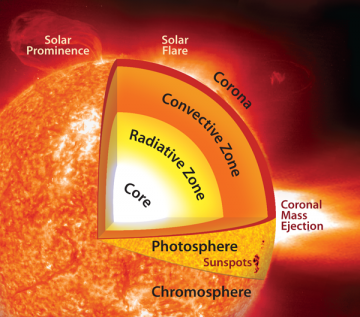
\includegraphics[width=0.65\textwidth]{figuras/SolarStructure.png}
\end{center}
\caption{Estructura interna del sol. Fuente: http://www.nasa.gov/.}
\label{estructura_solar}
\end{figure}

%Las manchas corresponden a concentraciones de flujo de campo magnético intenso, el que al estar tan concentrado inhibe el transporte de energía en esa zona y por ese motivo  la manchas tienen un brillo relativo inferior a las zonas sin manchas. Por lo general aparecen de a pares, donde cada miembro del par tiene polaridad magnética opuesta. El número de manchas que se observa en la fotósfera varía con el tiempo. A esta variación, aproximadamente periódica, se la conoce como el ciclo solar (ver Sección \ref{ciclo}). Las regiones del interior y superficie solar se esquematizan en la \fig{estructura_solar}, donde a su vez se muestra una representación de mancha solar en la fotósfera.

La corona solar es la atmósfera exterior del Sol, con una temperatura de 1 a 2 MK. Aunque la existencia de la corona se conoce desde hace mucho tiempo por los eclipses solares totales, su temperatura de un millón de grados no se reconoció hasta que sus espectros fueron interpretados correctamente por la física de los procesos de radiación en la década de 1940. Entonces se planteó la pregunta de por qué se produce una temperatura tan alta de la corona. Dado que la densidad de la corona ($10^{8} cm^{-3}$) es mucho menor que la de la fotosfera ($10^{17} cm^{-3}$), la densidad de energía térmica de la corona (aunque es 200–300 veces más caliente que la fotosfera) es insignificante en comparación con la densidad de energía fotosférica. 
Dado que no hay una fuente de energía plausible más lejos en la corona para calentar la misma, debemos asumir que existe algún mecanismo (lo mas probable es que sean varios coexistiendo) que transforme energía magnética en calor. Este es el problema del calentamiento coronal, aún sin resolver.

\begin{figure}[ht]
\begin{center}
%\includegraphics[width=0.99\textwidth]{figuras/solar_interior_nasa.jpg}
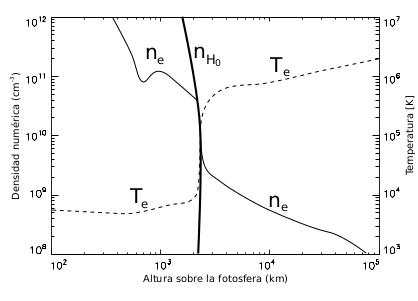
\includegraphics[width=0.65\textwidth]{figuras/calentamiento.png}
\end{center}
\caption{Esquema de la variación de densidad y temperatura con la altura de la atmósfera solar. La línea sólida denota la variación de la densidad de electrones, mientras que la línea a trazos indica la temperatura electrónica.}
\label{calentamiento}
\end{figure}



La Figura \ref{calentamiento} muestra las estructuras de temperatura y densidad de la atmósfera solar. Un límite delgado entre la cromosfera y la corona es llama región de transición, donde la temperatura salta repentinamente de $10^4$ K a $10^6 K$. La región de transición emite radiaciones ultravioleta (UV) y ultravioleta extrema (EUV). La emisión de la corona de 1–2 MK está en el EUV a rangos de rayos X suaves.
La última región es la corona que se extiende desde la región de transición hasta el medio interplanetario y se caracteriza por temperaturas del orden del MK y densidades del orden de $10^8\ - 10^9\ \rm {cm^{-3}}$. Varios fenómenos de interés astrofísico ocurren en distintas regiones de la corona como ser las eyecciones de masa coronal (CMEs por sus siglas en inglés) y las fulguraciones (\fig{estructura_solar}), etc.

\subsection{Viento solar}
Los movimientos convectivos debajo de la fotosfera generan campo magnético cuyas líneas atraviesan la corona. Gracias a la alta temperatura de la corona, los elementos que la componen se encuentran altamente ionizados y en consecuencia interactúan con el campo magnético del Sol. Como la divergencia del campo magnético es nula, las líneas de campo son cerradas, pero hay distintos tipos. Las más cortas se cierran cercanas cerca de la fotosfera y las más largas en el medio interplanetario, a estas últimas las llamaremos abiertas. Los arcos magnéticos influyen fuertemente en el plasma coronal, dejando materia ``atrapada'' en las líneas cerradas y eyectando materia al medio interplanetario siguiendo las líneas abiertas en lo que se llama {viento solar} . El viento solar invade el medio interplanetario, y junto con otros fenómenos como CMEs, tienen un impacto en la magnetósfera terrestre. El modelado y la predicción del clima espacial depende en buena parte de entender los fenómenos físicos que generan el viento solar.

El viento solar es plasma proveniente del sol, es el responsable de mantener la heliósfera y es el agente externo que moldea las magnetosferas planetarias. El viento solar se conforma de una componente altamente variable llamada viento solar lento con velocidades terminales de $\sim 450\pm 100$ km/s y densidades $\sim 10 \rm{ cm^{-3}}$ y se la asocia a regiones de campo magnético cerrado, y de una componente uniforme llamada viento solar rápido con velocidades $\sim 800\pm 100$ km/s y densidades $\sim 3 \rm{ cm^{-3}}$ y se la asocia a regiones de campo magnético abierto.

\begin{figure}[ht]
\begin{center}
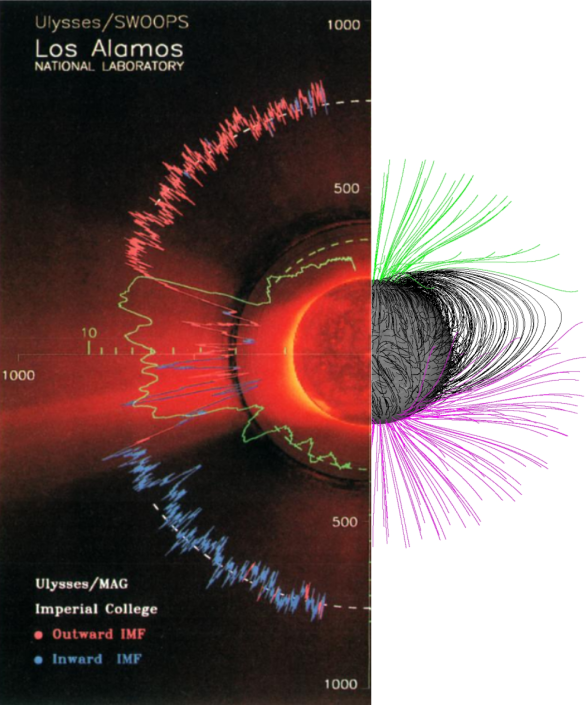
\includegraphics[width=0.85\textwidth]{figuras/mezcla_pfss_ulysses.png}
\end{center}
\caption{Izquierda: La velocidad del viento solar (en rojo y azul) y la densidad en verde, datos tomados con Ulysses. Derecha: líneas de campo magnético realizadas con un modelo potencial con superficie fuente. En negro las líneas magnéticamente cerradas y en verde y magenta las líneas abiertas con distinta polaridad.}
\label{ulysses}
\end{figure}

La Figura \ref{ulysses} muestra dos figuras en una. En la parte izquierda una porción de una figura del paper \citet{mccomas_2000} donde se muestran mediciones in situ de la órbita de Ulysses alrededor del Sol que salió de le eclíptica y paso por la zona polar. Se graficó en rojo y azul la velocidad del viento (cada color indica campo entrante o saliente), y en verde la densidad del viento. La figura de la derecha (creación propia) representa líneas de campo generadas con un modelo potencial con superficie fuente, donde se utilizó como dato un magnetograma (componente radial del campo magnético a nivel fotosférico) durante una época de mínimo de actividad solar. La figura muestra un campo magnético fuertemente dipolar (característico de un mínimo de actividad solar), las líneas negras son las denominadas líneas cerradas (también llamadas Streamer) y las líneas verde y magenta son líneas abiertas (con distinta polaridad). El plasma fluye por las líneas abiertas donde es acelerado y alcanza velocidades terminales altas y densidades bajas, en cambio en las líneas cerradas el campo queda atrapado mayormente y el plasma que escapa conforma el viento solar lento con menor velocidad y mayor intensidad. El objetivo de este trabajo es introducir los conceptos mas importantes para modelar la corona y el viento solar a gran escala.




\begin{comment}
\section{Magnetograma}

Los movimientos convectivos debajo de la fotósfera generan campo magnético cuyas líneas atraviesan la corona. Gracias a la alta temperatura de la corona, los elementos que la componen se encuentran altamente ionizados y en consecuencia interactúan con el campo magnético del Sol. Como la divergencia del campo magnético es nula, las líneas de campo generadas dentro del interior solar son cerradas, pero hay distintos tipos. Las más cortas se cierran cercanas cerca de la fotósfera y las más largas en el medio interplanetario, a estas últimas las llamaremos abiertas. Los arcos magnéticos influyen fuertemente en el plasma coronal, dejando materia ``atrapada'' en las líneas cerradas y eyectando materia al medio interplanetario siguiendo las líneas abiertas en lo que se llama \emph{viento solar} (ver Sección \ref{viento_solar}). El viento solar invade el medio interplanetario, y junto con otros fenómenos como CMEs, tienen un impacto en la magnetósfera terrestre. 

Debido al efecto dínamo y a las corrientes convectivas, el campo magnético solar varía considerablemente en el tiempo. Como consecuencia la corona y el viento solar varían, mostrando diferentes estructuras según la fase del ciclo en la cual el Sol se encuentra. 

El campo magnético coronal no es medible aún en forma directa ya que la sensibilidad instrumental requerida para una determinación de precisión razonable está aún lejos de alcanzarse. Sin embargo a nivel fotosférico la intensidad del campo magnético es lo suficientemente alta como para que el efecto Zeeman sobre las líneas de emisión provenientes de esa zona sean medibles con precisión. De esta forma el campo magnético es medido por magnetógrafos, los cuales proveen imágenes que describen la variación espacial de la intensidad del campo. A estas imágenes se las denomina magnetogramas. 



Los magnetogramas tradicionales proveen una medición de la componente del campo magnético a lo largo de la línea de visión. Esta medición es transformada en componente radial asumiendo que el campo es fundamentalmente radial en las cercanías de la fotósfera. Series de magnetogramas individuales tomados durante una rotación completa son combinados en los denominados \emph{magnetogramas sinópticos}, que proveen una descripcción de la la superficies solar en su totalidad. Los magnetogramas sinópticos pueden utilizarse para extrapolar el campo magnético en la corona solar. 

El modelo de extrapolación más {sencillo es el denominado potencial, que} asume una corona libre de corrientes y un valor de campo magnético radial en la fotósfera igual al brindado por el magnetograma. La condición de contorno exterior suele tomarse a $R = 2.5 \mrsun$ donde se asume campo magnético puramente radial. A la superficie esférica de radio $R$ se la denomina superficie fuente y a un modelo con estas características se lo llama modelo potencial con superficie fuente (o modelo PFSS, por sus siglas en inglés).

Matemáticamente el problema consiste en lo siguiente: dado el magnetograma sinóptico que define la componente radial del campo como $M(\theta,\phi)$ en $r=\mrsun$ y se debe encontrar el potencial escalar $\Phi$ tal que, $\nabla \cdot B = \nabla \cdot (\nabla \Phi)  = 0$, $\frac{\partial \Phi}{\partial r} (r=1\mrsun,\theta,\phi) = M(\theta,\phi)$ y $\Phi(r=R,\theta,\phi) = 0$, donde $\theta$ y $\phi$ son la co-latitud y la longitud, respectivamente. Este modelo es muy útil para tener una idea de la morfología del campo magnético hasta aprox 10 $\mrsun$ en un mínimo solar (donde la aproximación de corrientes nulas es mas creíble) y suele también usarse como condición inicial para modelos magnetohydrodinámicos (MHD). En esta monografía lo usaremos para ejemplificar la morfología del campo durante un mínimo y un máximo de actividad solar a modo de contexto.


\end{comment}

\begin{comment}
\section{Viento Solar}\label{viento_solar}
\textcolor{red}{
\begin{itemize}
\item Aceleración del viento solar, foco en la region abierta
\end{itemize}
}

El viento solar es plasma proveniente del sol, es el responsable de mantener la heliósfera y es el agente externo que moldea las magnetosferas planetarias. En las cercanías del Sol, el viento solar y el campo magnético rotan como un cuerpo rígido junto a él, y a medida que avanza hacia el medio interplanetario el viento y el campo magnético toman la forma de una espiral de Parker, como se explica mas adelante. El viento solar se conforma de una componente altamente variable llamada viento solar lento con velocidades terminales de $\sim 450\pm 100$ km/s y densidades $\sim 10 \rm{ cm^{-3}}$ y se la asocia a regiones de campo magnético cerrado, y de una componente uniforme llamada viento solar rápido con velocidades $\sim 800\pm 100$ km/s y densidades $\sim 3 \rm{ cm^{-3}}$ y se la asocia a regiones de campo magnético abierto. Estos valores son a 1 Unidad Astronómica (UA) y en el plano de la eclíptica, que es donde nos enfocaremos en este manuscrito ya que es donde se ubica el planeta Tierra. Existen, ademas, eventos transitorios como ejecciones de masa coronal que pueden influir en la estructura del viento solar que si bien suelen ser eventos de poca duración, su intensidad pueden afectar fuertemente a todo el medio interplanetario.


El primer modelo exitoso del viento solar se le atribuye a Parker \citep{parker_1958}, quien fue el primero en considerar un perfil de velocidad radial no nulo. El modelo asume: equilibrio ($\partial /\partial t =0$), gas formado por $e$ y $p$, neutralidad de carga, simetría esférica y temperatura constante. Como resultado, el perfil de velocidad logra aproximarse a las observaciones cerca del sol pero difiere mas allá de 1UA. Esto se mejora al introducir un perfil radial de temperatura que considera distintos fenómenos de aceleración por calentamiento. Para un desarrollo mas profundo dirigirse a \citet{prolss} (Capítulo 6.1.2).


Para entender la estructura de gran escala del viento solar debemos entender que la consideración de la simetría esférica del modelo de Parker es una simplificación. De hecho, continuos cambios son observados en las propiedades del viento solar durante una rotación solar. A lo largo de esta, la Tierra se ve embebida por momentos en regiones de viento solar rápido y otras de viento solar lento. Estas regiones están asociadas a agujeros coronales (AC) y a regiones con campo $B$ cerrado respectivamente. Cada región de la corona en el plano de la eclíptica emite su propio "sabor" de viento solar. Es decir que las partículas de VS de una región difiere en velocidad, densidad y temperatura de partículas de las originadas en otra región.


Para describir una estructura de gran escala de este viento solar inhomogeneo necesitamos saber la forma del flujo de distintos sectores asociados a {\rm jetlines}. Los jetlines conectan el flujo saliente del viento solar que se haya originado de una región fuente. Considerando que en la región fuente el VS inicia con velocidad radial ($\rm{u_{vs}}$) y que el propio sol rota sobre si mismo ($\Omega$), entonces cada jetline forma una espiral arquimediana como se indica en la \fig{espiral}. El ángulo entre un dado jetline y la dirección radial se puede aproximar como $\chi \sim arctan (\Omega .r /\rm{u_{vs}})$ y nos da valores de $\sim 45^{\circ}$ en la Tierra y alcanza los $\sim 90^{\circ}$ pasando Plutón. El viento solar (exceptuando regiones muy cercanas a la fotósfera) presenta presión de plasma mayor que la presión magnética, es decir $\beta=\frac{P_{gas}}{P_{mag}}=\frac{nk_BT}{B^2*\mu_0} >> 1$, esto es equivalente a despreciar el término difusivo en la Ecuación \ref{mhd_induccion}. En este régimen podemos considerar que las líneas de campo $B$ siguen al movimiento del plasma, de esta forma los flujos de plasma de un jetline no pueden atravesar jetlines vecinos. De esta forma regiones de viento solar rápido comprimen regiones de viento solar lento y se generan regiones de compresión y de rarefacción como se esquematiza en la figura \fig{espiral2} en el plano de la eclíptica visto desde el norte.


\begin{figure}[ht]
\begin{center}
%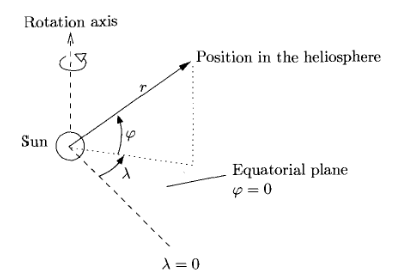
\includegraphics[width=0.55\textwidth]{figuras/coordenadas_sw.png}
%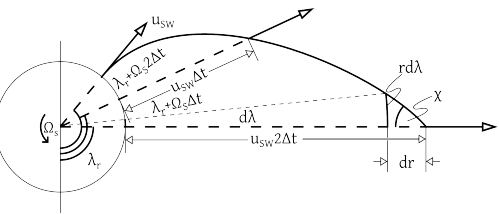
\includegraphics[width=0.75\textwidth]{figuras/espiral.png}
\end{center}
\caption{Arriba: Sistema de coordenadas heliosférico centrado en el sol (no co-rota con el sol). Abajo: evolución y morfología de un jetline con velocidad $u_{SW}$ constante.}
\label{espiral}
\end{figure}


En el artículo seleccionado que revisaremos en esta monografía se evaluaron distintas estructuras del viento solar: {\it high-speed streams} (HSS) que son básicamente corrientes de viento rápido proveniente de los AC, viento solar lento y transitorios que pueden ser provocados por ejecciones de masa coronal interplanetaria (ICMEs por sus siglas en inglés). El viento solar lento proviene de las regiones con líneas de campo cerradas, hay varios modelos que intentan explicarlo considerando velocidad y composición química. Si bien hay indicios, aún es tema que no esta cerrado. En la charla de la materia de esta monografía eh hablado de distintas fuentes del viento solar lento basándome en en el trabajo de \citet{suess_2009}.

\end{comment}
\chapter{Magnetohydrodinámica}\label{mhd}

La dinámica de los plasmas confinados magnéticamente, tal como se observa en los sistemas astrofísicos, es esencialmente de naturaleza macroscópica, por lo que se puede estudiar en el modo fluido, veremos a continuación este enfoque. 


La teoría cinética involucra detalles de las funciones de distribución que evolucionan en escalas de tiempo y duración muy cortas, como la longitud de Debye y la frecuencia de plasma. En este trabajo estamos interesados en la dinámica macroscópica de los plasmas magnetizados y bajo ciertas aproximaciones se puede obtener una descripción macroscópica utilizando promedios estadísticos. \textcolor{red}{Debemos considerar que la escala de tiempo en la que la descripción macroscópica es válida debe ser mayor que el tiempo que tarda en termalizar cada especie.}
%Para eso debemos considerar que la tasa de intercambio de energía entre dos partículas de la misma especie es mucho mayor que entre dos especies diferentes, la tasa de colisión entonces es considerada $\tau_{ii} \gg \tau_{ee} \gg \tau_{ei}$ (el subíndice  indica electrones y el subíndice i indica iones). 
El siguiente paso hacia la descripción macroscópica de un plasma es considerar escalas espaciales grandes (mucho mayor que el radio de ciclotron) y escalas temporales grandes (mucho mayor que la inversa de la frecuencia de ciclotron). Por último la dinámica del plasma debe ser mucho mayor que el tiempo de disipación del campo magnético (esto suele cumplirse incluso en escalas chicas). Con estas consideraciones es posible describir el fluido con un sistema de ecuaciones de dos fluidos, para combinarlos se define la densidad total de masa, la velocidad del centro de masa, la densidad de corriente, la presión y la densidad de carga como:

\begin{eqnarray}
  \rho &\equiv&  n_e m_e + n_i m_i \label{mhd_rho}\\
  \vec{v} &\equiv& (n_e m_e \vec{v}_e + n_i \textcolor{red}{m_i} \vec{v}_i) \label{mhd_v} \\
  \vec{j} &\equiv& -e(n_e \vec{v}_e + Z n_i \vec{v}_i) \\
  p &\equiv& p_e + p_i \label{mhd_p}\\
  \tau &\equiv& -e(n_e - Zn_i). \\
\end{eqnarray}
\textcolor{red}{Como última aproximación al enfoque MHD asumiremos cuasi neutralidad de carga $|n_e - Zn_i| \ll n_e$ y velocidades no relativistas $v \ll c$.}


La descripción física de un sistema hidrodinámico se realiza mediante las leyes de conservación para la masa (o densidad de masa, $\rho$), la densidad de momento ($\rho v$) y la densidad de energía del fluido (e). Este conjunto de leyes son las ecuaciones de Euler para fluidos no viscosos, o las de Navier–Stokes para un fluido viscoso. En el caso de un fluido conductor, las ecuaciones de Euler se acoplan con las ecuaciones de Maxwell, las cuales describen la evolución del campo electromagnético. Este enfoque nos permite tratar al plasma como un fluido simple conductor y se lo denomina Magnetohidrodinámica (MHD). En la aproximación MHD el plasma es tratado como un gas magnetizado conductor de corriente y eléctricamente neutro. Muchos de los aspectos físicos que caracterizan al plasma se pierden, sin embargo, la descripción es una buena aproximación para muchos problemas en los que los procesos son lentos, es decir en los que las frecuencias son mucho menores que la frecuencia de plasma y es el enfoque más utilizado para describir un plasma en la corona solar. %La teoría de un fluido (MHD) describe un plasma en términos de promedios macroscópicos, es decir, como funciones de posición y tiempo. Para que esta aproximación sea válida, el tamaño, la duración, la densidad y la intensidad del campo magnético deben ser tales que el comportamiento de fluido pueda representarse promediando los fenómenos microscópicos. La escala de tiempo debe ser mayor que el inverso de la frecuencia ciclotrónica, y la escala espacial debe ser mayor que el radio ciclotrónico. Además no se toman en cuenta los efectos de separación de cargas y la diferencia entre las temperaturas de electrones e iones.



\section{MHD ideal}\label{mhd_ideal}
%Desde la corona solar, pasando por el medio interplanetario y hasta el borde de la magnetosfera terrestre nos encontraremos con pasma caliente a baja densidad y embebido en campo magnético, el enfoque utilizado para estudiar los fenómenos que ocurren en un medio como este es utilizando magnetohidrodinámica (MHD).

%No es el objetivo de esta monografía hacer un desarrollo formal, pero sintetizaré brevemente las ecuaciones ya que nos dan contexto y serán de utilidad al hablar de reconexión magnética. Usaremos la aproximación de MHD ideal \citep{handbook_2007}, la cual consiste en carga total nula ($n_e = n_p$), fluidos no relativistas $\left| \frac{1}{c}\frac{\partial}{\partial t} \boldsymbol{E} \right| / \left| \nabla \times  \boldsymbol{B} \right| << 1$ y presión isótropa.
Las ecuaciones ideales de MHD describen el movimiento de un fluido perfectamente conductor que interactúa con un campo magnético. Por lo tanto, necesitamos combinar las ecuaciones de Maxwell con las ecuaciones de la dinámica de los gases y proporcionar ecuaciones que describan la interacción.

Primero consideremos las ecuaciones de Maxwell, que describen la evolución del campo eléctrico $\vec{E}(\vec{r},t)$ y el campo magnético $\vec{B}(\vec{r},t)$ en respuesta a la densidad de corriente $\vec{j}(\vec{r},t)$ y a la carga $\tau(\vec{r},t)$.
\begin{eqnarray}
\nabla \times \vec{E} &=& -\frac{\partial\vec{B}}{\partial t} \label{faraday}\\ 
\nabla \cdot \vec{B} &=& 0 \\
\nabla \times \vec{B} &=& \mu_0 \vec{J} + \frac{1}{c^2}\frac{\partial\vec{E}}{\partial t}\label{ampere}\\
\nabla \cdot \vec{E} &=& \frac{\tau}{\epsilon_0}. \label{poisson}\\
\end{eqnarray}

%donde estamos considerando fluidos no relativistas y por lo tanto despreciando la corriente de desplazamiento ($\frac{1}{c} \frac{\partial \vec{E}}{\partial t}$) en la ley de Ampere (Ec. \ref{ampere}).

Ahora consideremos la ecuación de la dinámica del gas para la evolución de la densidad $\vec{\rho}(\vec{r},t)$ y la presión $\vec{p}(\vec{r},t)$.
\begin{eqnarray}
\frac{d\rho}{dt} + \rho \nabla \cdot \vec{v} &\equiv& \frac{\partial \rho}{\partial t} +\nabla \cdot (\rho \vec{v}) = 0\\
\frac{d p}{dt} + \gamma p \nabla \cdot \vec{v} &\equiv& \frac{\partial p}{\partial t} + \vec{v} \cdot \nabla p + \gamma p \nabla \cdot \vec{v} = 0\\
\end{eqnarray}
donde utilizamos la definición de derivada convenctiva $\frac{d}{dt}=\frac{\partial}{\partial t} + \vec{v} \cdot \nabla$. 

Hasta el momento los dos sistemas de ecuaciones descriptos por las variables $\vec{E}, \vec{B}$ y por $\rho, p$ están desacopladas. Esta interacción se introduce a través de las ecuaciones que involucran el campo de velocidades $\vec{v}(\vec{r},t)$ del fluido. Dicha ecuación es el balance de fuerzas por unidad de volumen o conservación del momento dada por,

\begin{equation}
\rho \frac{d\vec{v}}{dt} = - \nabla p + \vec{J} \times \vec{B} +\rho \vec{g} +\tau \vec{E} \label{momento}
\end{equation}
que representa la aceleración causada por gravedad, gradiente de presión y contribuciones electromagnéticas.
Por último añadimos la ecuación del campo eléctrico de un fluido perfectamente conductor en movimiento,

\begin{equation}
\vec{E'} = \vec{E} + \vec{v} \times \vec{B} = 0 \label{campo_E}
\end{equation}
que expresa que el campo eléctrico $\vec{E'}$ en un marco comovil debe ser nulo.
En este punto el sistema de Ecuaciones (\ref{faraday})-(\ref{campo_E}) puede considerarse completo. Para el plasma que nos interesa a nosotros en este trabajo es suficiente con hacer algunas aproximaciones a estas ecuaciones. Vamos a considerar velocidades no relativistas $v\ll c$ y en ese caso podemos hacer las siguientes estimaciones al orden de magnitud de los diferentes términos de la ecuación de Ampere (Ec. \ref{ampere}).
\begin{equation}
\frac{1}{c^2} \left| \frac{\partial \vec{E}}{\partial t} \right| \sim \frac{v^2 B}{c^2 l_0} \ll \left| \nabla \times \vec{B} \right| \sim \frac{B}{l_0}
%\vec{E'} = \vec{E} + \vec{v} \times \vec{B} = 0 \label{campo_E}
\end{equation}
donde usamos que $v\sim l_0/t_0$ y que $E\sim v B$ (Ec. \ref{campo_E}). En consecuencia podemos despreciar la corriente de desplazamiento en la ley de Ampere.
Al mismo tiempo, la aproximación no relativista implica una simplificación en la ecuación de momentos (Ec. \ref{momento}), ya que

\begin{equation}
\tau \left| \vec{E} \right| \sim \frac{v^2}{c^2} \frac{B^2}{\mu_0 l_0} \ll \left| \vec{J} \times \vec{B}\right| \sim \frac{B^2}{\mu_0 l_0}
\end{equation}
donde hemos usado la Ec. \ref{ampere} habiendo despreciado la corriente de desplazamiento para el término de la derecha, y las Ecuaciones \ref{campo_E} y \ref{poisson} para el término de la izquierda. En consecuencia podemos despreciar la aceleración electrostática dada por las cargas y de esta forma eliminar la ecuación de Poisson (Ec. \ref{poisson}) de nuestro conjunto de ecuaciones.

De esta forma obtenemos las ecuaciones que componen MHD ideal:
\begin{eqnarray}
\frac{\partial \rho}{\partial t} +\nabla \cdot (\rho \vec{v}) = 0 \label{conserv_densidad} \\
%\rho \frac{d\vec{v}}{dt} = - \nabla p + \vec{J} \times \vec{B} +\rho \vec{g} +\tau \vec{E} \\
\rho \left( \frac{\partial\vec{v}}{\partial t} + \vec{v} \nabla \cdot \vec{v}\right) +\nabla p - \rho \vec{g} -\frac{1}{\mu_0}(\nabla \times \vec{B}) \times \vec{B} =0 \label{mhd_momento} \\
\frac{\partial p}{\partial t} + \vec{v} \cdot \nabla p + \gamma p \nabla \cdot \vec{v} = 0 \label{presion}\\
\frac{\partial \vec{B}}{\partial t} - \nabla \times (\vec{v} \times \vec{B}) = 0 \label{mhd_B} \\
\nabla \cdot \vec{B} = 0 \\
\end{eqnarray}
Estas conforman un conjunto de ocho ecuaciones diferenciales parciales no lineales para las ocho variables $\rho(\vec{r},t)$, $p(\vec{r},t)$, $\vec{v}(\vec{r},t)$ y $\vec{B}(\vec{r},t)$. Es de interés también elaborar las ecuaciones de evolución para las otras variables termodinámicas, que podrían reemplazar $\rho$ y $p$. Por ejemplo, la energía interna por unidad de masa $e$ (que es equivalente a la temperatura) y la entropía por unidad de masa $s$. Para este trabajo nos resultará útil la primera, que se define utilizando la ecuación de gases ideales $p = (n_e +n_i)kT$,
\begin{equation}
e \equiv \frac{1}{\gamma -1 } \frac{p}{\rho} \approx C_v T \label{ener}
\end{equation}

Si de la Ec. \ref{ener} reemplazamos $p=e (\gamma -1)\rho$ en la Ec. \ref{presion} y utilizamos la Ec. \ref{conserv_densidad} y multiplicamos la ecuación restante por $1/(\gamma -1)e$ obtenemos la ecuación para la energía interna (que reemplazaría a la Ec. \ref{presion} en el set de ecuaciones que conforman MHD ideal),

\begin{equation}
\frac{de}{dt} + (\gamma -1)e\nabla \cdot \vec{v} =0 \label{conserv_ener}
\end{equation}




\section{Leyes de conservación}\label{leyes_conserv}
A continuación expresaremos las ecuaciones que rigen MHD ideal en forma de leyes de conservación, es decir que deben poder escribirse como $\frac{\partial}{\partial t}(\cdot \cdot \cdot) +\nabla \cdot (\cdot \cdot \cdot) =0$.

Considerando el set de ecuaciones que conforman MHD ideal discutidos en la sección anterior y utilizando como variable la energía interna $e$ en lugar de la presión, es decir tomando en consideración la Ec. \ref{conserv_ener}, tenemos:

\begin{eqnarray}
\frac{\partial \rho}{\partial t} +\nabla \cdot (\rho \vec{v}) &=& 0 \label{mhd1}\\
\rho \frac{\partial\vec{v}}{\partial t} + \rho \vec{v} \cdot \nabla  \vec{v} +\nabla p - (\nabla \times \vec{B}) \times \vec{B} &=& -\rho \nabla \phi \label{momento2} \\
\frac{\partial e}{\partial t} + \vec{v}\cdot \nabla e +(\gamma -1)e\nabla \cdot \vec{v} &=& 0 \label{ener_int} \\
\frac{\partial \vec{B}}{\partial t} + \nabla \times \vec{E} &=& 0  \label{fara_1}\\
\nabla \cdot \vec{B} &=& 0 \\
\vec{E} &=& -\vec{v}\times \vec{B} \label{mhd6} 
\end{eqnarray}
Donde hemos utilizado un potencial gravitatorio ($\vec{g}=-\nabla \phi$) en la ecuación de momento. Cabe notar que hemos eliminado la constante $\mu_0$ por conveniencia. Las unidades mks pueden reobtenerse haciendo el siguiente cambio de variable $\vec{B}\rightarrow \vec{B}/\sqrt{\mu_0}$, $\vec{E}\rightarrow \vec{E}/\sqrt{\mu_0}$ y $\vec{j}\rightarrow \vec{j}\sqrt{\mu_0}$. De ahora en más obviaremos la constante.

En este punto solo la conservación de la masa y el campo magnético tienen la forma de ecuación de conservación, a continuación veremos brevemente como obtener la ecuación de conservación del momento y de la energía total.

Los primeros dos términos de la ecuación de momento pueden reescribirse como
\begin{equation}
  \rho \frac{\partial\vec{v}}{\partial t} + \rho \vec{v} \cdot \nabla \vec{v} = 
  \frac{\partial}{\partial t}(\rho \vec{v}) + \vec{v} \nabla \cdot(\rho \vec{v})=
  \frac{\partial}{\partial t} (\rho \vec{v}) + \nabla \cdot (\rho \vec{v} \vec{v})
\end{equation}
donde en la primer igualdad se utilizó la conservación de la masa y en la segunda se utilizó la identidad \ref{apen_1} (ver apéndice). El último término puede escribirse como
\begin{equation}
  -\vec{J} \times \vec{B} = \vec{B} \times (\nabla \times \vec{B}) = \nabla (\frac{1}{2}B^2)  - \nabla \cdot (\vec{B}\vec{B}) 
\end{equation}
donde en la segunda igualdad es necesario utilizar las identidades \ref{apen_2} y \ref{apen_4}. Esto nos permite reescribir la ecuación de momento en forma de conservación como se indica en la Ec. \ref{conserv_momento}. El segundo término de la ley de Faraday puede ser reescrito haciendo uso de la Ec. \ref{campo_E} y de la identidad \ref{apen_3} 
\begin{equation}
  \nabla \times \vec{E} = - \nabla \times (\vec{v} \times \vec{B})= \nabla \cdot (\vec{v}\vec{B} -\vec{B}\vec{v} ),
\end{equation}  
lo que nos permite escribirla en su forma conservativa (Ec. \ref{conserv_bflux}).
Por otro lado la ecuación de energía interna no puede ser llevada por si sola a una forma conservativa debido a que solo contiene una parte de la energía que puede ser convertida en otras formas de energía. A continuación obtendremos entonces la ecuación de conservación para la energía total, lo cual se logra añadiendo las distintas contribuciones de energía cinética, interna y magnética.

Si multiplicamos $\vec{v} \cdot$  Ec. \ref{momento2} 
\begin{eqnarray}
\rho \vec{v}\cdot (\frac{\partial \vec{v}}{\partial t}+\vec{v \cdot \nabla \vec{v}})+\vec{v} \cdot \nabla p -\vec{v}\cdot \vec{j}\times \vec{B}= - \rho \vec{v} \cdot \nabla \phi
\end{eqnarray}
redistribuyendo los primero términos y utilizando la ecuación de conservación de masa obtenemos,
\begin{eqnarray}
  \frac{\partial}{\partial t} (\frac{1}{2}\rho v^2) + \nabla \cdot  (\frac{1}{2}\rho v^2 \vec{v}) +\vec{v} \cdot \nabla p - \vec{v} \cdot (\vec{j} \times \vec{B}) = - \rho \vec{v} \cdot \nabla \phi.
\end{eqnarray}

Multiplicando $\rho$ Ec. \ref{ener_int} 
\begin{eqnarray}
   \rho \frac{\partial e}{\partial t} +\rho \vec{v} \cdot \nabla e + (\gamma -1 )pe \nabla \cdot \vec{v} =0
\end{eqnarray}
y utilizando la conservación de masa se obtiene,
\begin{eqnarray}
   \frac{\partial}{\partial t} (\rho e) +\nabla \cdot (\rho e \vec{v}) + p \nabla \cdot \vec{v} =0.
\end{eqnarray}

Finalmente tomando $\vec{B} \cdot$ Ec. \ref{fara_1} 
\begin{eqnarray}
  \vec{B} \cdot \frac{\partial \vec{B}}{\partial t} - \vec{B} \cdot \nabla \times (\vec{v}\times \vec{B})=0
\end{eqnarray}
y utilizando las identidades \ref{apen_5} y \ref{apen_6} obtenemos,
\begin{eqnarray}
     \frac{\partial}{\partial t} (\frac{1}{2} B^2) + \nabla \cdot \left[ \vec{B} \cdot \vec{B}\vec{v} -\vec{v}\cdot\vec{B}\vec{B} \right] + \vec{v} \cdot \vec{j} \times \vec{B} = 0
\end{eqnarray}

Estas últimas tres expresiones para los tres términos de la energía conforman la ecuación de conservación de la energía total (Ec. \ref{energia}). De esta manera obtenemos la forma conservativa de las ecuaciones de MHD en la aproximación ideal\footnote{\citet{goedbloed_2004}}:

\begin{eqnarray}
\frac{\partial \rho}{\partial t} +\nabla \cdot (\rho \vec{v}) = 0\\ \label{conserv_d}
\frac{\partial}{\partial t}(\rho \vec{v}) + \nabla \cdot \left[ \rho \vec{v}\vec{v} + (p+\frac{1}{2}B^2) \vec{I} - \vec{B}\vec{B} \right] = - \rho \nabla \phi   \label{conserv_momento}
\end{eqnarray}

\begin{equation}
\begin{split} 
 \frac{\partial}{\partial t} (\frac{1}{2}\rho v^2 &+ \rho e +\frac{1}{2} B^2) +\\ 
& \nabla \cdot \left[ (\frac{1}{2}\rho v^2 + \rho e + p + B^2) \vec{v} -\vec{v}\cdot \vec{B}\vec{B}  \right] = -\rho \vec{v} \cdot \nabla \phi +\textcolor{red}{Q_{nocons}} \label{energia}
\end{split}
\end{equation}
\begin{eqnarray}
\frac{\partial \vec{B}}{\partial t} + \nabla \cdot (\vec{v}\vec{B} -\vec{B}\vec{v} ) = 0\\ \label{conserv_bflux}
\nabla \cdot \vec{B} = 0 
\end{eqnarray}
las cuales representan la conservación de masa, momento, energía total y flujo magnético respectivamente. Si consideramos que no hay fuentes ni pérdidas de energía, es decir que no hay términos no conservativos en la Ec. \ref{energia} ($Q_{nocons} = 0$), entonces las ecuaciones \ref{conserv_d}-\ref{energia} representan las ecuaciones de conservación MHD que modelan un plasma compuesto por iones y electrones. Esta representación no alcanza para modelar correctamente la corona solar, ya que modela viento solar con velocidades muy lentas y provee perfiles de densidad incorrectos, es decir que el viento a 1 UA no concuerda con las mediciones in-situ hechas por satélites como Ulysses \citep{mccomas_2000}.

Añadiremos al modelo, en la Sección \ref{seccion_perdida}, las principales pérdidas de energía relevantes en la corona solar. Luego en la Sección \ref{seccion_alfven} incluiremos términos de inyección de energía tanto para electrones como iones.

%diativa y conductiva (necesarias para el balance hidrostático dentro de un arco coronal, ver \citet{aschwanden_2004}) y para acelerar el viento solar se deben considerar términos de inyección de energía. En la Sección \ref{seccion_perdida} ahondaremos en este punto.




\subsection{Funciones de pérdida de energía} \label{seccion_perdida}
El término $Q_{nocons}$ en la Ec. \ref{energia} representa los términos no conservativos que afectan a la energía, incluyendo términos de pérdida y de ganancia energética. Estos términos no conservativos dependerán del fenómeno u entorno físico que se pretenda modelar. Dado que nuestro caso de interés es la extensión de la corona solar hasta el medio interplanetario, entonces mencionaremos a continuación los términos de pérdida principales que deben ser incluidos a la hora de modelas el viento solar. 


Por un lado tenemos la tasa de pérdida de energía radiativa en la baja corona que es proporcional al producto de la densidad electrónica e iónica, multiplicada por la función de pérdida radiativa que es una función dependiente de la temperatura $\Lambda(T)$
\begin{equation}
  Q_{rad} = N_e N_i \Lambda(T_e). \label{qrad}
\end{equation}


En pérdidas debemos agregar el término de flujo de calor de electrones $\nabla \cdot \vec{q_e}$, que consiste en una contribución no colisional y otra colisional. En los casos en los que la densidad es relativamente alta se utiliza la formulación colisional dada por Spitzer \citep{spitzer_1953}
\begin{equation}
   \vec{q}_{e,col} = - k_e T_e ^{5/2}\vec{b}\vec{b} \cdot \nabla T_e, \label{qe_col}
\end{equation}
donde $\vec{b}=\vec{B}/B$ indica la dirección del campo magnético y $k_e$ es la constante de Spitzer con unidades de $erg^{-1} cm^{-1} K^{7/2}$. En el caso de baja densidad predomina el flujo de electrones no colisional donde podemos utilizar la expresión de flujo sugerida por \citet{hollweg_1978},

\begin{equation}
   \vec{q}_{e,no-col} \sim p_e \vec{v}. \label{qe_nocol}
\end{equation}



En el caso de considerar una fuente de energía para electrones o para iones entonces debemos agregar los términos correspondientes $Q_e$ y $Q_i$ en la parte derecha de la Ec. \ref{energia}. {Comentaremos mas sobre esto en la Sección \ref{seccion_alfven} donde asignaremos a estos términos la transferencia de energía por disipación de ondas de Alfvén.}


\begin{comment}
Ley de Ohm
\begin{equation}
\vec{J} = \sigma (\vec{E} + \frac{\vec{v} \times \vec{B}}{c}) \label{ohm_resis}
\end{equation}
donde en el límite difusivo consideramos $\sigma \rightarrow \infty$, obteniendo
\begin{equation}
\vec{E} = -\frac{1}{c} \vec{v} \times \vec{B}
\end{equation}

El balance de fuerzas por unidad de vlumen o conservación del momento viene dado por
\begin{equation}
\rho \frac{d\vec{v}}{dt} = - \nabla p + \vec{J} \times \vec{B} -\rho \vec{g} \label{momento}
\end{equation}
donde se usa la definición de derivada convenctiva $\frac{d}{dt}=\frac{\partial}{\partial t} + \vec{v} \cdot \nabla$. El segundo término de la derecha es la fuerza de Lorenz y puede escribirse en función del tensor de esfuerzos de Maxwell $\vec{J}\times\vec{B}=\nabla \cdot \boldsymbol{T}$ con $\boldsymbol{T} = \frac{1}{\mu_0}\vec{B}\vec{B}-\frac{B^2}{2\mu_0}\boldsymbol{I}$. El primer término representa a la tensión magnética, que se opone a la deformación de las líneas de campo y el segundo término representa la presión magnética. 


Conservación de la densidad de energía
\begin{equation}
\frac{\partial e}{\partial t}+ \nabla \cdot [\vec{v}(e+p)] = \vec{J} \cdot \vec{E}
\end{equation}
donde el término de la derecha representa la tasa de calor producida por la corriente óhmica, y se definió la energía por unidad de volumen como
\begin{equation}
  e = c_v p +\frac{1}{2}\rho v^2+\frac{B^2}{2}
\end{equation}
\textcolor{red}{definir como se obtuvo esta ecuacion, dmitruk/aschwanden}
\end{comment}

%Utilizando la ley de Ampere (Ec. \ref{ampere}) reescribimos la conservación de la energía y del momento, como:
%\begin{eqnarray}
%\frac{\partial e}{\partial t}+ \nabla \cdot [\vec{v}(e+p)] = \vec{B}(\vec{v}\cdot \vec{B})-(\vec{v}\cdot\vec{B}))\nabla \cdot \vec{B} \\
%\rho \frac{d\vec{v}}{dt} = - \nabla p + (\nabla \cdot (\vec{B}\vec{B})-\nabla \cdot (\vec{B}^2/2)\boldsymbol{I} -\vec{B}(\nabla \vec{B})    )-\rho \vec{g}
%\end{eqnarray}
%donde se utilizó la identidad $\vec{A}\times(\vec{B}\times\vec{C})=(\vec{A}\vec{C})\vec{B}-(\vec{A}\vec{B})\vec{C}+(\vec{C}\vec{A})\vec{B}-(\vec{B}\vec{A})\vec{C}$

\section{Inducción magnética}
En el caso de MHD ideal hemos despreciado el término disipativo. Si bien las ecuaciones de de MHD ideal obtenidas en la Sección \ref{mhd_ideal} permiten una generalización directa para incluir el término disipativo debido a la resistividad del plasma, no nos resultará útil obtener las ecuaciones de MHD resistivo. En cambio introduciremos la ecuación de inducción magnética que nos permitirá mas adelante entender como se transfiere energía de por disipación de ondas de Alfvén.

Si tomamos la ley de Ohm (Ec. \ref{campo_E}) considerando el término resistivo tenemos,
\begin{equation}
\vec{E'} = \vec{E} + \vec{v} \times \vec{B} = \eta \vec{j} \label{campo_E_resis}
\end{equation}
donde ahora se tiene en consideración la disipación Ohmica a través de la resistividad $\eta$ del plasma.
Reemplazando la Ec. \ref{campo_E_resis} y la ley de Ampere (Ec. \ref{ampere}) en la ley de Faraday (Ec. \ref{faraday}) obtenemos la ecuación de inducción magnética
\begin{equation}
\frac{\partial \vec{B}}{\partial t} = \nabla \times (\vec{v} \times \vec{B}) + \eta \nabla^2 \vec{B}. \label{induccion}
\end{equation}
%donde hemos definido la constante de difusión magnética como $\eta = c^2/4\pi \sigma$. 
La evolución del campo magnético y de velocidades viene dado por las ecuaciones \ref{momento} y \ref{induccion}, que se encuentran fuertemente acoplados y tiene términos no lineales.
Se puede estimar la importancia de la resistividad comparando los dos términos, para ello definimos el número de Reynold magnético como:
\begin{equation}
R_m = \frac{\nabla \times (\vec{v} \times \vec{B}) }{\eta \nabla^2 \vec{B}} \approx \frac{vL}{\eta}\label{reynold}
\end{equation}
 donde L es una longitud característica de la variación espacial del campo magnético. Cuando el fluido esta en reposo o bien cuando las velocidades son pequeñas, predomina el segundo término de la derecha en la ecuación de inducción. Esto implica que una configuración inicial del campo magnético disminuirá con un tiempo de difusión $t_d\approx L^2/\eta$. Este tiempo de difusión es mucho mas grande que el observado en estructuras de la corona solar, lo que indica que la disipación es acelerada por otro mecanismo.
 
Por otro lado, cuando la difusividad es baja, es decir $R_m$ grande, la Ec. \ref{induccion} se lee como $\frac{\partial \vec{B}}{\partial t} = \nabla \times (\vec{v} \times \vec{B})$ y expresa la conservación del flujo magnético (reobtenemos la Ec. \ref{conserv_bflux}) que atraviesa una curva cerrada que se mueve con la velocidad local del fluido. De esto se desprende que el fluido arrastra a las líneas de campo y se dice entonces que el campo magnético está ``congelado'' al fluido. La noción de las líneas de campo arrastradas por el fluido son solo una imagen pictórica, ya que las líneas de campo son una idealización, que indica la dirección del campo local en un instante. El hecho de que las líneas sean arrastradas corresponde a que se generan corrientes que modifican el campo para que su dirección (instante a instante) cambie. A la congelación del campo a la materia se la conoce como teorema de Alfvén.
\begin{comment}
\textcolor{red}{
Podemos ver que el flujo de  líneas de campo magnético se conserva al integrar la ley de Ohm sobre una curva cerrada e igualandola con la forma integral de la ley de Faraday, obtenemos
\begin{equation}
  \oint_{C} (\vec{E}+\vec{v}\times \vec{B})\, d\vec{r} =\eta \oint_{C} \vec{J} \, d\vec{r} = - \frac{d}{d} \int_S \vec{B} \, d\vec{S}
\end{equation}
y en el límite de conductor perfecto (MHD ideal) sin difusión obtenemos
\begin{equation}
\frac{d}{dr} \oint_S \vec{B} d\vec{S} = 0 \, ,   \,   \,   \,  \eta \rightarrow 0,
\end{equation}
 y de esta forma el flujo se conserva.
 La derivada convectiva de un elemento de fluido es la siguiente
\begin{equation}
  \frac{d}{dt} d\vec{r} = \vec{v}(\vec{x} + d\vec{r})-\vec{v}(\vec{x})=(d\vec{r}\cdot \nabla) \vec{v}, 
\end{equation}
donde $d\vec{r}$ representa un diferencial de elemento de fluido que se desplaza desde $\vec{x}$ a $\vec{x}+d\vec{r}$.
La misma ecuación define el campo magnético sin difusión,
\begin{equation}
  \frac{d}{dt} \vec{B} = (\vec{B}\cdot \nabla) \vec{v}. 
\end{equation}
De esta forma podemos notar que $\vec{B}$ y $d\vec{r}$ estan gobernados por la misma ecuación, y por lo tanto deben evolucionar de la misma manera, es decir que las líneas de campo $\vec{B}$ evolucionan igual que las líneas materiales.
}
%\textcolor{red}{Por lo tanto, el flujo magnético a través de un elemento de superficie que se mueve conjuntamente es constante. Pero, dado que esto es válido para cualquier elemento de la superficie, se conserva el flujo a través de cualquier superficie limitada por un contorno C que se mueve con el fluido.}

\textcolor{red}{para que pongo esto?}
\end{comment}



\section{Ondas de Alfvén}\label{seccion_alfven}

Para abordar el problema del calentamiento coronal existen principalmente dos ramas de investigación en la actualidad, por un lado calentamiento por nanofulguraciones, que transfieren energía desde la cromosfera hacia la base de los arcos coronales, 

El calentamiento coronal es hasta hoy en día un tema abierto. La imposibilidad de realizar mediciones in-situ en las proximidades de la fotosfera ralentizan el avance en esta área. Distintos fenómenos físicos que se saben ocurren en la corona coexisten simultáneamente y liberan energía calentando la corona y acelerando el viento solar, por ejemplo reconexión magnética, nanofulguraciones, disipación de ondas de Alfvén, etc. Veremos a continuación esta última y como implementarla en nuestro modelado de la corona y además como introducirlo en en las ecuaciones de conservación MHD que mencionamos anteriormente.


En un plasma existen distintos tipos de ondas, en particular si despreciamos la gravedad en las ecuaciones de MHD ideal, las ondas resultan de perturbaciones del campo presión, densidad, velocidad y campo magnético. Cada tipo de onda tiene asociada su correspondiente relación de dispersión y es producida por una fuerza restitutiva. %Veremos a continuación las onda magnéticas compresionales denominadas ondas de Alfvén.

Cuando una línea de campo magnético se ve deformada debido a fluctuaciones en el campo de velocidades, la curvatura resultante da lugar a tensión de Faraday (fuerza restitutiva, $\sim B^2$) que tiende a enderezar la línea. Dado que para $R_m >> 1$ las líneas están congeladas a la materia, se podría considerar que hay cierta inercia y por lo tanto parece intuitivo esperar ondas transversales en el campo magnético. 




Para ilustrar esta idea consideraremos una perturbación $\delta \rho, \delta \vec{v},\delta p, \delta \vec{B}$ pequeñas con respecto a su estado base $\rho,  \vec{v}, p$ y $\vec{B}$. Reemplazamos las perturbaciones en las ecuaciones de MHD ideal y linealizando obtenemos:

\begin{eqnarray}
  \frac{\partial}{\partial t} \delta \rho_0 &=& - \rho_0 \nabla \cdot \delta \vec{v}\\
  \rho_0 \frac{\partial}{\partial t} \delta \vec{v} &=& -\nabla \delta p + (\nabla \times \delta \vec{B})\times \vec{B_0} \label{pertu1}\\
  \frac{\partial}{\partial t} \delta p &=& -\gamma p_0 \nabla \cdot \delta \vec{v}\\
  \frac{\partial}{\partial t} \delta \vec{B} &=& \nabla \times (\delta \vec{v}\times \vec{B_0}) \label{pertu2}.  
\end{eqnarray}
La primera ecuación que determina $\delta \rho$ esta desacoplada. Considerando que estamos interesados en las perturbaciones magnéticas, podemos elegir $p=0$ y de esta forma queda definido $\delta p=0$. Tomando la derivada temporal de la \textcolor{red}{Ec. \ref{pertu1}} y reemplazando en ella la Ec. \ref{pertu2} obtenemos una ecuación de onda para la perturbación en velocidad:
\begin{equation}
  \rho_0 \frac{\partial^2 \delta \vec{v}}{\partial t^2}=\Bigg(\nabla \times \frac{\partial \delta \vec{B}}{\partial t} \Bigg) \times \vec{B_0}= \vec{B_0} \times \Bigg( \nabla \times \Bigg( \nabla \times (\vec{B_0}\times \delta \vec{v}) \Bigg) \Bigg).
\end{equation}
Utilizando como solución una onda plana
\begin{equation}
  \delta \vec{v}(\vec{r},t)=V e^{i(\vec{k}\vec{r}-wt)}
\end{equation}
se obtienen como solución ondas transversales ($\delta\vec{v}\perp \vec{B}_0$) que se propagan en al dirección del campo magnético ($\vec{k} \parallel \vec{B}_0$). Estas ondas tienen la relación de dispersión $w=\pm k_{\parallel} v_A$  donde se define la velocidad de Alfvén como  $v_A=\frac{\vec{B}_0}{\sqrt \mu_0 \rho_0}$. Las ondas de Alfvén son causadas por la tensión de las líneas de campo magnético, las cuales tienden a restaurar la forma inicial.


\subsection{Disipación de ondas de Alfvén}

Con el objetivo de introducir la ecuación para energía de onda, resulta de utilidad introducir las variables de Elsässer\footnote{\citet{elsasser_1950}}:

%Para ilustrar esta idea consideraremos una perturbación respecto de un equilibrio estático con campo magnético uniforme utilizando las variables de Elsässer, a saber:
\begin{equation}
  \vec{z}^\pm = \vec{v} \pm \frac{\vec{B}}{\sqrt{\mu \rho}}.
\end{equation}
%donde el signo positivo indica propagación en la misma dirección que el campo magnético y el signo negativo en dirección opuesta.
Haciendo uso de estas variables y considerando incompresibilidad ($\nabla \cdot \vec{v}=0$) es posible reescribir el sistema de ecuaciones (\ref{mhd1}) - (\ref{mhd6}) de la siguiente forma:

\begin{eqnarray}
  \frac{\partial \vec{z}^+}{\partial t}+ \vec{z}^- \cdot \nabla \vec{z}^+ &=& -\nabla(p + \vec{B}^2/2\mu) \label{pertu11} \\
  \frac{\partial \vec{z}^-}{\partial t}+ \vec{z}^+ \cdot \nabla \vec{z}^- &=& -\nabla(p + \vec{B}^2/2\mu)\\
  \nabla \cdot \vec{z}^\pm &=& 0. \label{pertu3}
\end{eqnarray}
%Los pasos detallados de la reescritura de las ecuaciones MHD en variables de Elsässer pueden encontrarse en \citet{elsasser_1950}. En este punto la única consideración realizada es incompresibilidad ($\nabla \cdot \vec{v}=0$).

Proponemos pequeñas perturbaciones ($\delta$) en el campo de velocidad y el campo magnético sobre el equilibrio (dado por $v_0 = 0; B=B_0$), es decir $\vec{B} = \vec{B}_0 + \delta \vec{B}$ y $\vec{v} = 0 + \delta \vec{v}$ y reescribimos las variables de Elsässer,

\begin{equation}
  \vec{z}^\pm = \textcolor{red}{\vec{z}^\pm + \tilde{\vec{z}}^\pm} = \pm V_{A0} + \vec{\delta v} \pm \frac{\vec{\delta B}}{\sqrt{\mu \rho_0}}
\end{equation}
donde $V_{A0} = \vec{B}_0/\sqrt{\rho \mu_0}$ es la velocidad de Alfvén.
Reemplazando esta nueva variable con perturbaciones en las ecuaciones (\ref{pertu11})-(\ref{pertu3}) y luego fijando por un lado $\vec{z}^+ \neq 0 ,\vec{z}^- =0$ y por el otro $\vec{z}^+ =0 ,\vec{z}^- \neq 0$ (es decir considerando ondas en una sola dirección) obtenemos dos ecuaciones desacopladas,

\begin{eqnarray}
  \frac{\partial \vec{z}^+}{\partial t} &=& - V_{A0}\nabla \vec{z}^+ \, \, \, \, ;\vec{z}^- = 0,\\
  \frac{\partial \vec{z}^-}{\partial t} &=&  V_{A0}\nabla \vec{z}^- \, \, \, \, ;\vec{z}^+ = 0.
\end{eqnarray}

Estas ecuaciones describen que las variables de Elsässer en un marco de incompresibilidad representan ondas de Alfvén que se propagan paralela o anti paralelamente al campo magnético \citep{magyar_2019}. %Para una descripción mas detallada de la naturaleza de las variables de Elsässer en MHD referirse a \citet{magyar_2019}.
 %\textcolor{red}{Veremos en la Sección \ref{chap_awsom} la importancia en el calentamiento coronal que poseen las ondas contrapropagantes.}

La ecuación para la densidad de energía de onda viene dada por $w_\pm = \rho \vec{z}^2_\pm /4$. Para una sola onda propagante (es decir sin considerar una onda contrapropagante), la ecuación de la evolución de la energía en estos casos es,
\begin{equation}
  \frac{\partial w_\pm}{\partial t} + \nabla \cdot [(\vec{v}\pm \vec{V}_A)w_\pm] = - \frac{w_\pm}{2}(\nabla \cdot \vec{v}) ,\label{alfven_1}
\end{equation}
donde los términos de la izquierda describen la propagación de las ondas de Alfvén a lo largo de las líneas de campo magnético y el término de la derecha representa la reducción de la densidad de energía dada en la expansión del plasma. Una descripción completa de la ecuación la densidad de energía de las ondas turbulentas de Alfvén utilizando la aproximación Wentzel–Kramers–Brillouin puede encontrarse en \citet{vander_2014}.%, donde se parte de una perturbación en el campo de velocidades y campo magnético en las ecuaciones \ref{momento2} y \ref{fara_1}, luego se utilizan las variables de Elsässer y finalmente considerando una sola onda propagante se obtiene la Ec. \ref{alfven_1}.

%Las ondas de Alfvén que se propagan a lo largo de las líneas de campo mangnético hacia afuera

La disipación de la onda de Alfvén ocurre cuando interactúan dos ondas que se propagan en direcciones opuestas, esto se da naturalmente en la corona baja, a lo largo de líneas magnéticamente cerradas.
La reflexión de la onda de Alfvén a partir de gradientes de densidad es el proceso físico que da como resultado la reflexión de onda en las líneas magnéticamente abiertas, manteniendo así una fuente de ambos tipos de ondas en ambos casos. Esta interacción entre onda propagante y contrapropagante genera una cascada turbulenta y disipación de la energía (\citet{hollweg_1986}; \citet{dmitruk_2002}). Para explicar esta disipación haremos uso de la descripción fenomenológica de disipación de Kolmogorov descripta en la Sección \ref{turbulencia}.

La tasa de disipación de densidad de energía es controlada por la amplitud de la onda propagante en sentido opuesto $|\vec{z_-} = 2 \sqrt{w_/\rho}|$ y por una longitud de correlación (L) entre las ondas. De esta forma introducimos a la derecha de la Ec. \ref{alfven_1} el término disipativo,

\begin{equation}
  \frac{\partial w_\pm}{\partial t} + \nabla \cdot [(\vec{v}\pm \vec{V}_A)w_\pm] = - \frac{w_\pm}{2}(\nabla \cdot \vec{v}) - \Gamma_{\pm} \textcolor{red}{ w_\pm},\label{alfven_2}
\end{equation}
donde
\begin{equation}
  \Gamma_{\pm} = \frac{2}{L}\sqrt{\frac{w_{\mp}}{\rho}}.
\end{equation}

En el caso de incorporar calentamiento de ondas de Alfvén al modelo MHD, la energía disipada en la Ec. \ref{alfven_2} debe balancear las fuentes de energía de iones y electrones ($Q_i$ y $Q_e$) que debemos agregar a la derecha de la ecuación de balance de energía (Ec. \ref{energia}), es decir

\begin{equation}
  Q_i +Q_e = \Gamma_+ w_+ + \Gamma_- w_-
\end{equation}
donde se entiende que $Q_i + Q_e$ es la disipación total. El particionamiento de la disipación es un tema abierto, algunos enfoques pueden encontrarse en \citet{hollweg_1986} y \citet{vander_2014}.

Las ondas de Alfvén ejercen presión isotrópica (ver Ec. 21 en \citet{jacques_1977}), la relación entre la presión de onda y la densidad de energía de onda es $P_A = (w_+ + w_-)/2$. Esta presión aporta en la aceleración del viento solar y debe ser considerada en la ecuación de momento (Ec. \ref{momento}) junto con los otros términos de presión isótropa. De esta forma, siguiendo los pasos para la obtención de las ecuaciones de conservación mencionado en la Sección \ref{leyes_conserv}, el término $p_A$ aparecerá en las ecuaciones de conservación del momento (Ec. \ref{conserv_momento}) y de la energía (Ec. \ref{energia}), detalladas explícitamente en la Sección \ref{chap_awsom}.

% es decir: $\nabla \cdot \left[ (p+\frac{1}{2}B^2 +P_A )\vec{I} \right]$.



{En este modelo utilizaremos la disipación de las ondas de Alfvén como el proceso físico que impulsa el viento solar y calienta el plasma coronal.}


%\textcolor{red}{donde $B_0$ y $p_0$ son valores constantes y las perturbaciones son ondas planas $\delta\vec{B},\delta{v} \sim exp^{i(\vec{k}\vec{r}-wt)}$ Utilizando estas perturbaciones en las Ecuaciones \ref{momento} y \ref{induccion} se obtienen como solución, ondas transversales ($\delta\vec{B}\perp \vec{B}_0$, $\delta\vec{v}\perp \vec{B}_0$) que se propagan en al dirección del campo magnético ($\vec{k} \parallel \vec{B}_0$). Estas ondas tienen la relación de dispersión $w=\pm k v_A$  donde se define la velocidad de Alfvén como  $v_A=\frac{\vec{B}_0}{\sqrt \mu_0 \rho_0}$. Las ondas de Alfén son causadas por la tensión de las líneas de campo magnético, las cuales tienden a restaurar la forma inicial.}



%Damping of Alfvén wave turbulence as a source of coronal heating has also been extensively studied from the early days of in situ solar wind observations (e.g., Barnes 1966, 1968). Later, it was demonstrated that reflection from sharp pressure gradients in the solar wind (Heinemann and Olbert 1980; Leroy 1980) is a critical component of Alfvén wave turbulence damping (Matthaeus et al. 1999; Dmitruk et al. 2002; Verdini and Velli 2007). For this reason, many numerical models explore the generation of reflected counter-propagating waves as the underlying cause of the turbulence energy cascade (e.g., Cranmer and Van Ballegooijen 2010), which transports the energy of turbulence from the large-scale motions across the inertial range of the turbulence spatial scale to short-wavelength perturbations. The latter can be efficiently damped due to wave–particle interaction. In this way, the turbulence energy is converted to random (thermal) energy.




\section{Calentamiento por turbulencia MHD} \label{turbulencia}

Introduciremos a continuación una descripción fenomenológica de la transferencia de energía mediante la cual la turbulencia generada por las ondas de Alfvén disipa energía. No se pretende en este trabajo hacer un desarrollo extenso de este tema, sino mas bien dar una idea mas bien fenomenológica de lo que conforma la base de la teoría de la cascada de energía de Kolmogorov para pequeñas escalas. El desarrollo formal para hidrodinámica puede encontrarse en \citet{kolmogorov_1941} y una explicación mas amigable en \citet{davidson_2013}.


%\textcolor{red}{Concepto de cascada de energía de Kolmogorov.}\\
En la mayoría de flujos turbulentos con $Re$ grandes, donde un forzado entrega energía al sistema a una cierta escala ($L_i$), la disipación no ocurre eficientemente en esas mismas escalas. La energía pasa primero de vórtices grandes a otros mas pequeños en múltiples pasos. Digamos que de los vórtices de inyección $L_i$ pasa a $L_0$, luego a $L_1$ y así sucesivamente hasta $L_n$ ($L_i>L_0>L_1>...>L_n$), donde finalmente la energía cinética es transformada en calor.
Cuando $R=vL/\eta >>1$ las fuerzas viscosas que actúan en vórtices con escalas L mucho mas grandes que $L_n$ son despreciables y la cascada se da por inercia (domina el término inercial en la ecuación de inducción, Ec. \ref{induccion}). Este proceso se detiene cuando las fuerzas viscosas son del mismo orden que el término inercial, donde la energía cinética puede ser convertida eficientemente en calor como se esquematiza en el diagrama de la Figura \ref{kolmogorov}. La cascada entonce se detiene cuando alcanza la micro escala $L_n$ que debe satisfacer $L_n \eta/ \nu \sim 1$. Se puede pensar a la cascada de energía como una series de inestabilidades sucesivas debidas a los términos no lineales entre las escalas de inyección $L_i$ y las disipativas $L_n$, alcanzando finalmente un balance entre la energía que ingresa al sistema y la que se disipa.


\begin{figure}[ht]
\begin{center}
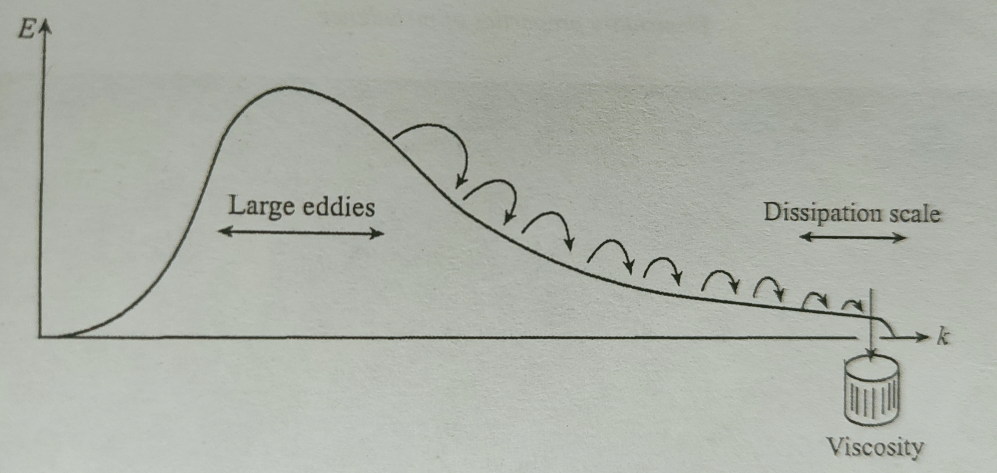
\includegraphics[width=0.55\textwidth]{figuras/kolmogorov.png}
\end{center}
\caption{Diagrama esquemático de la cascada de energía de Kolmogorov (Extraído de la Sección 8.4 del libro \citet{davidson_2013}.}
\label{kolmogorov}
\end{figure}





\chapter{Modelo solar por calentamiento de ondas de Alfvén} \label{chap_awsom}
Esfuerzos recientes apuntan a desarrollar y testear modelos MHD que incluyan a las ondas de Alfvén como el agente impulsor principal tanto para calentar el plasma como para acelerar el viento solar \citep{gombosi_2018}. En este contexto se desarrolló el modelo Alfvén Wave Solar Model (AWSoM;  \citet{vander_2014}). Este modelo MHD 3D de la corona solar es parte del Space Weather Modeling Framework (SWMF; \citet{swmf_2005}), y toma como único dato el campo magnético mediante magnetogramas, es decir la medición fotosférica de la componente radial del campo magnético. El modelo utiliza un conjunto de ecuaciones MHD que obtendremos a continuación (Ec. \ref{awsom_1}-\ref{awsom_e}) utilizando todo lo mencionado en las secciones anteriores y modela en forma tridimensional tanto la corona como la heliósfera interna.


Tal como fue introducido en la Sección \ref{seccion_alfven} y \ref{turbulencia}, este modelo aborda calentamiento de la corona solar al incluir la interacción no lineal de las ondas de Alfvén desde la cromosfera hacia el exterior y contrapropagadas (reflejadas) en las líneas magnéticamente cerradas lo que da como resultado una cascada turbulenta. Dentro de los agujeros coronales, no hay líneas de campo magnético cerradas, por lo tanto, no hay ondas de propagación opuesta. En cambio, un reflejo de las ondas que se propagan hacia el exterior (dada por gradientes de densidad) genera localmente ondas que se propagan hacia el Sol. Estas ondas contrapropagantes conducen a una tasa de disipación de turbulencia en los agujeros coronales generando calentamiento y acelerando el viento solar rápido.

Esta energía turbulenta disipada se distribuye entre protones y electrones utilizando teorías de amortiguación de onda lineal y calentamiento estocástico. El modelo incluye enfriamiento radiativo y la conducción de calor de electrones tanto colisional como no colisiona,l introducida en la Sección \ref{seccion_perdida} y no utiliza funciones de calentamiento ad-hoc.

Las ecuaciones que resuelve el modelo son:

\begin{eqnarray}
\frac{\partial \rho}{\partial t} +\nabla \cdot (\rho \vec{v}) = 0\\ \label{awsom_1}
\frac{\partial \vec{B}}{\partial t} + \nabla \cdot (\vec{v}\vec{B} -\vec{B}\vec{v} ) = 0\\ \label{awsom_2}
\frac{\partial}{\partial t}(\rho \vec{v}) + \nabla \cdot \left[ \rho \vec{v}\vec{v} + (p_i +p_e +p_A+\frac{1}{2}B^2) \vec{I} - \vec{B}\vec{B} \right] = - \rho \frac{GM_{\odot}}{r^3} \vec{r} \label{awsom_3}\\
\nabla \cdot \vec{B} = 0, \label{awsom_4}
\end{eqnarray}
donde, $\rho$ es la densidad de masa definida en la Ec. \ref{mhd_rho}, $\vec{v}$ es la velocidad definida en la Ec.  \ref{mhd_v}, $\vec{B}$ es el campo magnético, G es la constante gravitacional, $M_{\odot}$ es la masa solar, $\vec{r}$ es el vector posición relativo al centro del Sol, $p_A$ es la presión que ejercen las ondas de Alfvén y hemos diferenciado la presión (Ec. \ref{mhd_p}) en su componente iónica y electrónica. Al separar estas presiones isotrópicas podemos separar la ecuación de conservación de la energía (Ec. \ref{energia}) tanto para iones como electrones,  


\begin{equation}
\begin{split} 
 \frac{\partial}{\partial t} \Bigg( \frac{1}{2}\rho v^2 + \frac{p_i}{\gamma -1} &+\frac{1}{2} B^2 \Bigg) + \\
 \nabla \cdot & \left[ \Bigg( \frac{1}{2} \rho v^2 + \frac{ \gamma p_i}{ \gamma -1} + B^2 \Bigg) \vec{v} -\vec{v}\cdot  \vec{B}\vec{B}  \right] =\\
  &-\rho \frac{GM_{\odot}}{r^3}\vec{r}\vec{v}  + \frac{N_i k_b}{\tau_{ei}}(T_e - T_i) + Q_i  \label{awsom_i}
\end{split}
\end{equation}

\begin{equation}
\begin{split} 
 \frac{\partial}{\partial t} \Bigg( \frac{p_e}{\gamma -1} \Bigg) + 
 \nabla \cdot \Bigg( \frac{\gamma p_e}{\gamma -1}\vec{v} \Bigg) &+ \nabla \cdot \Bigg( p_A \vec{v} \Bigg) =\\
  -\nabla \cdot \vec{q_e} &+\frac{N_i k_b}{\tau_{ei}}(T_i - T_e) -Q_{rad} +Q_e  \label{awsom_e}
\end{split}
\end{equation}

Al separar las especies debemos introducir el intercambio de energía por colisión Coulombiana entre los iones y electrones, donde $\tau_{ei}$ es el tiempo de relajación  y $k_B$ es la constante de Boltzmann. El modelo considera la ecuación de estado de gases ideales para ambas especies, $p_{e,i}= N_{ei}k_B T_{e,i}$ y el índice politrópico $\gamma = 5/3$. El término $Q_{rad}$ representa la tasa de pérdida radiativa (Ec. \ref{qrad}) en la corona ópticamente delgada.

Para incorporar la componente colisional y no colisional del flujo de calor de electrones mencionadas en la Sección \ref{seccion_perdida} que involucre una transición suave a medida que nos alejamos del Sol el modelo utiliza

\begin{equation}
  \vec{q}_e = f_S \vec{q}_{e,col} + (1-f_S) \vec{q}_{e,no-col}
\end{equation}
donde se utiliza la fracción de Spitzer $f_S$ definida en función de la distancia heliocéntrica como
\begin{eqnarray}
  f_S = \frac{1}{1+(r/r_H)^2}
\end{eqnarray}
donde $r_H =5 R\odot$ es un valor fijo. De esta forma cerca del Sol ($r/R_h <1$), donde los valores de densidad son relativamente altos, vale $f_S \sim 1$ y predomina el flujo colisional de Spitzer. Por el contrario, lejos del Sol ($r/R_h >1$), donde los valores de densidad son relativamente bajos, vale $f_S \rightarrow 0$ y predomina el flujo no colisional de Hollweg.


Las funciones de calentamiento de electrones e iones se indican mediante $Q_e$ y $Q_i$, respectivamente. Su suma es igual a la disipación total de turbulencia dada por ondas de Alfvén por unidad de tiempo y por unidad de volumen, que queda determinada por la ecuación de la densidad de energía de ondas de Alfvén (Ec. \ref{alfven_2}).

Notar que la consistencia del modelo se manifiesta explícitamente en el hecho de que la suma de las ecuaciones de energía de ondas de Alfvén Ec. \ref{alfven_2}, energía iónica Ec. \ref{awsom_i} y energía electrónica Ec. \ref{awsom_e} tiene forma de ley de conservación. Donde quedarían del lado derecho las fuentes no conservativas, que no tienen forma de divergencia, y que se deben a las pérdidas de energía por emisión y por el trabajo realizado contra la fuerza gravitacional.  



\begin{equation}
\begin{split} 
 \frac{\partial}{\partial t} \Bigg( \frac{\rho v^2}{2} + \frac{p_i + p_e}{\gamma -1} &+\frac{B^2}{2} +w_+ + w_-\Bigg)  \\
 + \nabla \cdot  &\left[ \Bigg( \frac{\rho v^2}{2} + \frac{ \gamma (p_i+p_e)}{ \gamma -1} + B^2 \Bigg) \vec{v} -\vec{v}\cdot  \vec{B}\vec{B}  \right] \\
 +\nabla \cdot & [(w_+ + w_-+p_A)\vec{v} + (w_+ -w_-)\vec{V}_A]\\
=-\rho & \frac{GM_{\odot}}{r^3} \vec{r}\vec{v}  - Q_{rad} -\nabla \cdot \vec{q_e}  \label{awsom_final}
\end{split}
\end{equation}


Desde el grupo de Física Solar del Instituto de Astronomía y Física del Espacio\footnote{\url{http://iafe.uba.ar}} llevamos a cabo distintos frentes de investigación en colaboración con el Departamento de Clima y Ciencias Espaciales e Ingeniería (CLaSP\footnote{\url{https://clasp.engin.umich.edu}}, por sus siglas en inglés) en la Universidad de Michigan (EEUU), donde el modelo AWSoM fue desarrollado.

El grupo CLaSP proveyó el set de datos para una rotación reciente y perteneciente al último mínimo de actividad. Esto nos proporciona un Sol en su estado mas simple y sencillo para su análisis. Veremos a continuación algunos resultados para la rotación de Carrington (CR) 2223 que tuvo lugar entre el 16 de Octubre y el 12 de Noviembre del 2019, período en el cual el Sol se encontraba en un mínimo de actividad\footnote{\url{http://solarcyclescience.com/forecasts.html}}. 





\subsection{Resultados MHD}

Se utilizó como único dato un magnetograma ADAPT-GONG (componente radial de $B$ a $1R_{\odot}$). Debido a que CR 2223 se encuentra en un mínimo de actividad, el modelo muestra un campo magnético mayormente dipolar a toda altura. A modo de ejemplificación de algunos de los resultados que provee el modelo 3D, seleccionamos mapas de latitud en función de longitud (llamados mapas de Carrington) para una altura especifica. Una forma de visualizar esto, es considerar al set de datos 3D como una cebolla, donde cada capa es una altura diferente. Cada capa esférica puede desplegarse en un mapa de Carrington, el caso análogo mas conocido es el mapa planisferio de la Tierra.


\begin{figure}%[ht]
\begin{center}
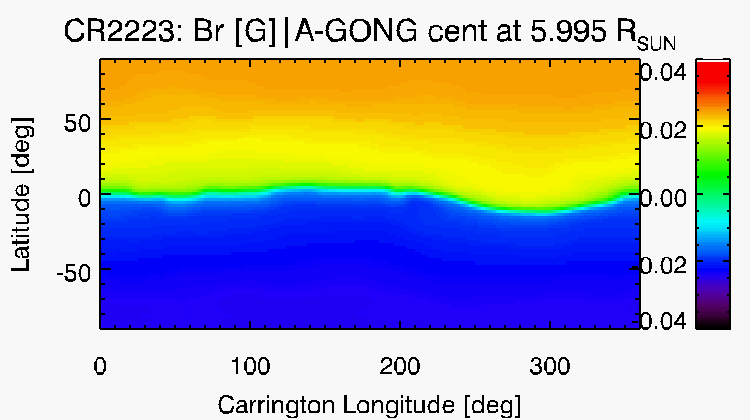
\includegraphics[width=0.75\textwidth]{figuras/map_Br_awsom_2223_cocent_extended_5_995_Rsun.png}
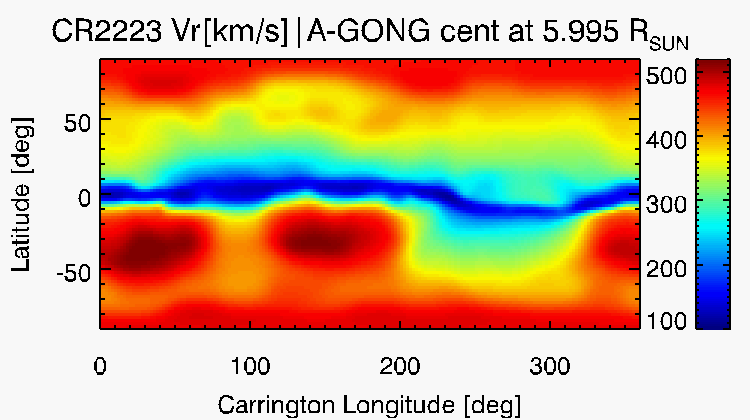
\includegraphics[width=0.75\textwidth]{figuras/map_Vr_awsom_2223_cocent_extended_5_995_Rsun.png}
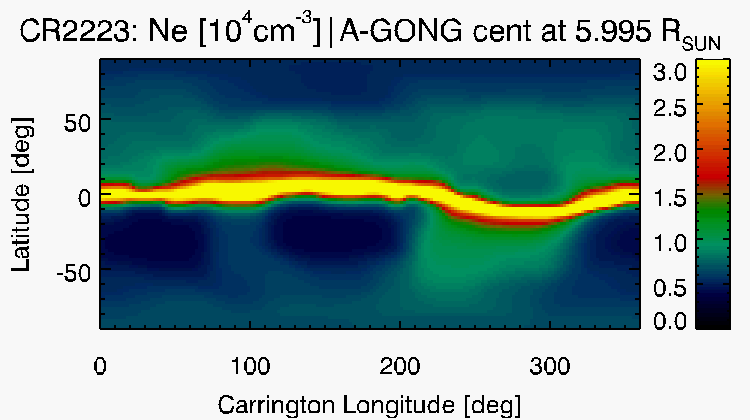
\includegraphics[width=0.75\textwidth]{figuras/map_Ne_awsom_2223_cocent_extended_5_995_Rsun.png}
\end{center}
\caption{Resultados del modelo AWSoM para CR2223 a $6 R_{\odot}$. Arriba se muestra un mapa de Carrington de componente radial del campo magnético, en el medio un mapa de Carrington de la componente radial de la velocidad del viento solar y abajo un mapa de Carrington de la densidad electrónica.}
\label{resultados1}
\end{figure}

Se ejemplifica en la Figura \ref{resultados1} mapas de Carrington de la componente radial de campo magnético (arriba) y de la componente radial de la velocidad del viento solar (abajo) a la altura de $6 R_{\odot}$. En la primera se puede ver claramente la forma dipolar de $B_r$. El hecho de que la región de cambio de polaridad del campo se encuentre cerca del ecuador es debido a que la rotación es de un mínimo de actividad, a esta región se la conoce como Hoja de Corriente Heliosférica (HCS, por sus siglas en inglés). El mapa de velocidad  del viento (medio de la figura) muestra un mínimo en la zona de la HCS, lo que conforma el viento solar lento. A medida que nos desplazamos desde latitudes ecuatoriales hacia los polos, la velocidad aumenta hasta alcanzar su máximo en la zona polar, conformando el viento solar rápido. Si bien a esta altura aún no se alcanzó la velocidad terminal ya se observa la relación 2:1 entre el viento rápido y el lento. El mapa de densidad electrónica $N_e$ a la misma altura. El modelo muestra densidades máximas en la HCS y mínimas en la zona polar. Estos resultados son consistentes con un viento solar lento y denso asociado al Streamer ecuatorial y un viento solar rápido y más tenue en la zona polar asociado a los agujeros coronales.

La Figura \ref{resultados2} muestra un mapa de Carrington la presión de onda Alfvén a bajas alturas. La zona mas oscura que denota relativamente baja presión se da dentro de la zona magnéticamente cerrada, y en rojo se muesta la zonas abiertas donde la presión es relativamente mas alta. Este mapa deja en evidencia que la disipación de ondas de Alfvén acelera el viento rápido, proveniente de la zona polar.


\begin{figure}%[ht]
\begin{center}
%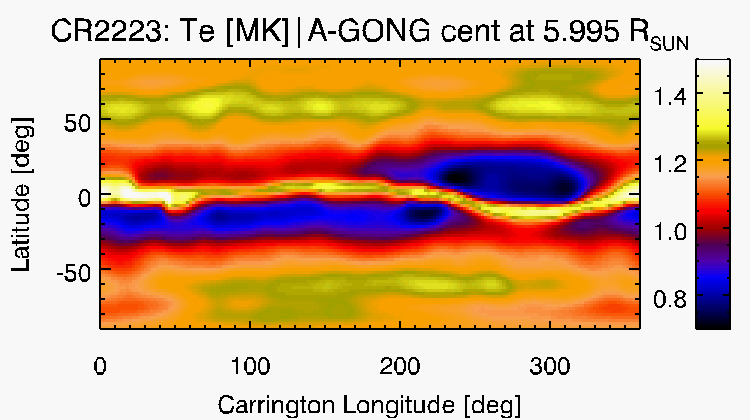
\includegraphics[width=0.75\textwidth]{figuras/map_Te_awsom_2223_cocent_extended_5_995_Rsun.png}
%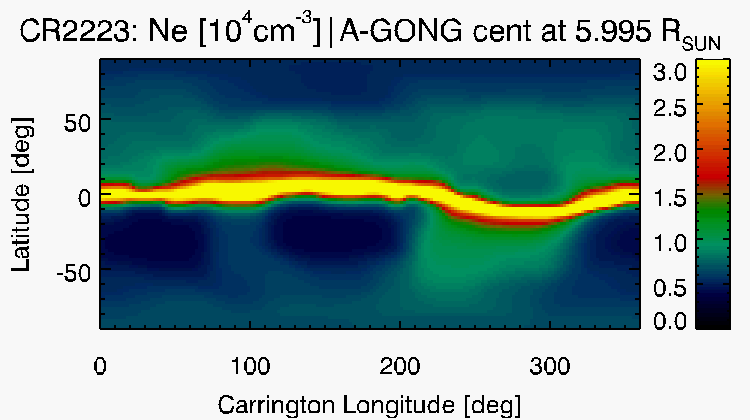
\includegraphics[width=0.75\textwidth]{figuras/map_Ne_awsom_2223_cocent_extended_5_995_Rsun.png}
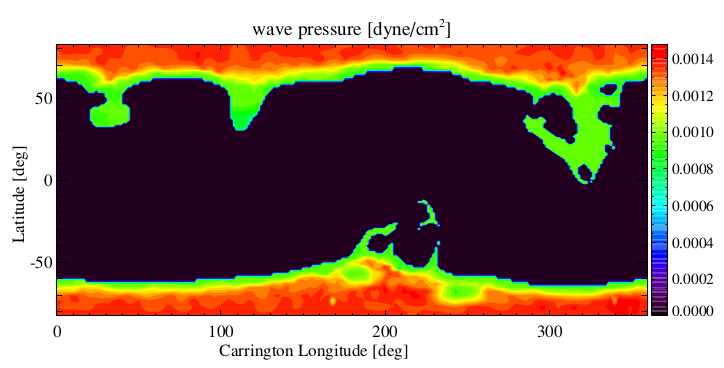
\includegraphics[width=0.75\textwidth]{figuras/presion_alfven_vander2010.png}
\end{center}
\caption{Mapa de Carrington de la presión de onda de Alfvén a $1.03 R_{\odot}$}
\label{resultados2}
\end{figure}

En conclusión:
Una cascada de energía turbulenta hacia escalas de pequeña longitud puede sostenerse gracias a ondas Alfvén reflejadas por la densidad media y los gradientes del campo magnético. Este mecanismo deposita energía de manera eficiente en la corona inferior. Esto proporciona un mecanismo de calentamiento robusto que puede explicar las altas temperaturas coronales observadas, explica la aceleración del viento en las zonas abiertas y explica la distribución significativa del calentamiento (por unidad de volumen) por debajo de $2R_\odot$ necesarios en los modelos del origen del viento solar.


El modelo AWSoM es puesto a prueba y validado con observaciones a medida que incorpora mas física (\citet{oran_2015}, \citet{sachdeva_2019}, \citet{lloveras_2020}, \citet{lloveras_2020BAAA}, etc.). Actualmente se está llevando a cabo un análisis comparativo de la densidad electrónica entre el modelo MHD y tomografía en luz blanca con datos del coronógrafo LASCO-C2. La presente monografía proveyó los fundamentos físicos para proponer una comparación energética entre el modelo MHD y un enfoque hidrostático utilizando datos tomográficos con datos en Extremo Ultravioleta obtenidos tomados por AIA. Ambos análisis formarán parte de la tesis de doctorado. 




%Los elementos ad hoc pueden eliminarse del modelo de corona solar asumiendo que el plasma coronal se calienta por la disipación de la turbulencia de la onda de Alfvén. La disipación en sí es causada por la interacción no lineal entre ondas que se propagan de manera opuesta. Dentro de los agujeros coronales, no hay líneas de campo magnético cerradas, por lo tanto, no hay ondas de propagación opuesta. En cambio, un reflejo débil de las ondas que se propagan hacia el exterior genera localmente ondas que se propagan hacia el sol, tal como lo cuantificaron van der Holst et al. (2014). La pequeña potencia en estas ondas de propagación hacia el interior generadas localmente (y disipadas casi de inmediato) conduce a una tasa de disipación de turbulencia reducida en los agujeros coronales, lo que naturalmente da como resultado la estructura del viento solar bimodal.

%El modelo Alfvén Wave Solar Model (AWSoM por sus siglas en inglés, \citet{vander_2014}) es un modelo MHD-3D que considera temperaturas protónicas y las temperaturas electrónicas de la corona solar y la heliosfera interna y proporciona la distribución 3D de densidad y temperaturas, así como también la estructura magnética 3D y velocidad del viento solar. 



%\textcolor{red}{Dado que el ensanchamiento de la región de transición empuja la corona hacia afuera, el modelo AWSoM logra condiciones coronales a una altura  1.05 R, por debajo de la cual los resultados no pueden compararse con las reconstrucciones tomográficas coronales. Para impulsar el modelo AWSoM, las estimaciones del campo magnético fotosférico del Sol son la entrada principal. Los magnetogramas sinópticos se utilizan para especificar las condiciones iniciales y de contorno del campo magnético. Usamos el modelo PFSS para extrapolar el campo magnético 3D (de los mapas de campo magnético fotosférico 2D) usando armónicos esféricos. Se considera que la superficie de la fuente está a 2,5 R. GONG proporciona mapas de superficie sinópticos de disco completo del componente del campo magnético radial del Sol. Sin embargo, dado que las regiones polares no se observan bien desde la eclíptica, GONG estima los campos polares ajustando un polinomio a las latitudes observadas vecinas, lo que podría conducir a inexactitudes. El modelo ADAPT (Worden y Harvey, 2000) proporciona una mejora con respecto a estos mapas, que crea mapas sinópticos sincrónicos mediante la incorporación de supergranulación, circulación meridional y rotación diferencial. Estos mapas proporcionan una descripción basada en la física de los campos magnéticos polares no observados (Arge et al., 2010; Henney et al., 2012). En este trabajo, utilizamos el mapa sinóptico de GONG como entrada para CR 2082 (los mapas ADAPT-GONG no están disponibles para CR 2082) y el mapa de campo magnético global ADAPT-GONG para CR 2208. Con base en los resultados de esfuerzos anteriores, para CR 2082 el El campo magnético del mapa GONG se escala en un factor de 1,85 para campos débiles (B r <5 G), mientras que no se aplica ninguna modificación en el caso del mapa ADAPT-GONG para CR 2208. El conjunto de simulación de estado estable AWSoM -up y los parámetros de entrada para ambas rotaciones se describen a continuación.}










%\chapter{comparacion/validacion modelo}
%\textcolor{red}{
%\begin{itemize}
%  \item comentar que el modelo ha sido validado en trabajos previos mediante observaciones.
%  \item se plantea hacer un analisis energetico comparando con un modelo hidrostatico isotermico aplicado a %DEMT.
%\end{itemize}
%}

%\section{Enfoque hisdrostático}
%\section{DEMT}
%\section{AWSoM vs DEMT}

\chapter{Apéndice}
\begin{eqnarray}
  \nabla \cdot (\vec{a}\vec{b}) &=& \vec{a} \cdot \nabla \vec{b} + \vec{b}\nabla \cdot \vec{a} \label{apen_1}\\ 
  \vec{a} \times (\nabla \times \vec{b}) &=& (\nabla \vec{b})\cdot \vec{a}- \nabla \cdot (\vec{a}\vec{b})-\vec{b}\nabla \cdot \vec{a}  \label{apen_2}\\
  \nabla \times(\vec{a} \times \vec{b}) &=& \nabla \cdot (\vec{b}\vec{a}-\vec{a}\vec{b}) \label{apen_3}\\
  \nabla (\vec{a}\cdot \vec{b}) &=& (\nabla\vec{a})\cdot \vec{b}+(\nabla\vec{b})\cdot \vec{a} \label{apen_4}\\
  \nabla \cdot (\vec{a} \times \vec{b}) &=& \vec{b} \cdot \nabla \times \vec{a} - \vec{a} \cdot \nabla \times \vec{b} \label{apen_5} \\
  \vec{a}\times (\vec{b} \times \vec{c}) &=& \vec{a} \cdot \vec{c}\vec{b} - \vec{a}\cdot \vec{b}\vec{c} \label{apen_6}
\end{eqnarray}






\bibliographystyle{spr-mp-sola}
\bibliography{bibliografia}

\end{document}






%\footnote{Para un desarrollo formal referirse al apunte de Fernando Minotti en la páguina web de la UBA, http://materias.df.uba.ar/plasma2019c2/files/2019/11/PLASMA\_2019.pdf}





